\chapter{Multi-task learning for extrapolation}
\label{chapMultiTaskExtrapolation}

\begin{mdframed}[hidealllines=true,backgroundcolor=lightgray!20]
\section*{Résumé}
Dans la partie \ref{partIncorporateMultipleOutputs}, nous nous intéressons à l'apprentissage de relations entre plusieurs sorties. Une régression sur les sorties multiples peut être divisé en deux catégories, lorsque nous souhaitons découvrir des relations sur plusieurs sorties, et lorsque nous voulons appliquer une relation connue entre les sorties (en tant que biais) dans notre algorithme d'apprentissage.

Dans ce chapitre, nous verrons comment effectuer la régression GP en présence de sorties multiples. Une méthode simple d'apprentissage d'un modèle de régression pour les sorties multiples est de supposer le nombre de sorties comme une dimension supplémentaire (cette dimension supplémentaire est une variable catégorielle). Cette hypothèse est bénéfique pour deux raisons, nous avons effectivement augmenté le nombre de points de données (figure \ref{figoutputsAsAnExtraDimension}), puis des fonctions de covariances pour plusieurs dimensions (section \ref{secMultiDimensionalKernels}) peuvent être également appliquées au cas des sorties multiples (section \ref{subsecAnExtraDimension}).

Si aucune information n'est disponible sur la relation entre les sorties, nous pouvons apprendre la relation entre les sorties en utilisant une covariance `simple MTGP’ (section \ref{simpleMultiTask}), un `Linear Model Of Coregionalization' (section \ref{subsecLMC}), ou un `convoluted GP’ \cite{alvarez2011kernels}. Si nous savons \textit{a-priori} que les sorties proviennent de modèles de fidélité multiples, nous pouvons utiliser la fonction de covariance jointe proposée par \cite{kennedy2000predicting} (section \ref{secMultiFidelityMTGP}).

Dans la section \ref{subsecMTGPExtrapolation}, nous avons montré comment les modèles GP multi-fidélité peuvent être utilisés pour effectuer une interpolation ou une extrapolation des données expérimentales du modèle. Nous incluons un terme d'erreur et un terme de translation dans un modèle multi-fidélité normal pour tenir compte des différences entre le modèle de simulation et les données expérimentales. Dans des travaux futurs, nous souhaitons quantifier la performance des différentes méthodes d'extrapolation et décider de la méthode à choisir dans un scénario particulier.
\end{mdframed}


%\pagebreak

\section{Introduction}

In the current part (part \ref{partIncorporateMultipleOutputs}) we are interested in learning relationships between multiple outputs. Performing regression on multiple-outputs can be split into two categories, first when we wish to discover relationships across multiple outputs, and second when we wish to enforce a known relationship between outputs (as a bias) into our learning algorithm.

\marginnote{\textsl{Multi-Task Learning}}[1cm]
When no relationship is known between outputs, we are interested in discovering these relationships. Several real-world problems often exhibit strong correlations between output variables, for example, correlations across spatial coordinates ($x, y, z$) in an experiment. This setting is also called `Multi-Task Learning' in the machine learning literature. Learning relationships across outputs can improve the efficiency and prediction accuracy of the models when compared to training the outputs individually. This is because learning together outputs which are related, effectively increases the number of data-points, thereby providing more data for the learning algorithm  \cite{caruana1998multitask}. In the GP literature these models are called `Multi-Task GP' (MTGP) \cite{alvarez2011kernels, bonilla_multi-task_2008, Boyle05dependentgaussian}, while in the kriging literature they are called as Cokriging \cite{helterbrand1994universal, chiles1999geostatistics, ver1998constructing}.

\marginnote{\textsl{Enforcing relationships}}[1cm]
\sloppy
When a relationship between the outputs is known, enforcing such a relationship in a learning algorithm will mean that we have implemented a correct bias. The outputs can be results from computer codes of varying accuracy \cite{kennedy2000predicting, forrester2007multi, le2013multi}, they can be related through a known equation\footnote{For example if we know that $acceleration = d(velocity)/d(time)$ and we measure both velocity and acceleration. How can we enforce the known equation into our model?} \cite{ginsbourger2013invariances, sarkka2011linear}, or they can be related through a known computer code\footnote{For example stress and forces in a CSM code} \cite{Constantinescu2013}. 

We split the part \ref{partIncorporateMultipleOutputs} of this thesis into two chapters. The current chapter (chapter \ref{chapMultiTaskExtrapolation}) will describe the basics of MTGP, present a model to interpolate a series of multi-fidelity simulations, and then propose a method to extrapolate experimental data in the presence of simulation models. The next chapter (\ref{chapAddingEquationsInGP}) will describe how to encode known relationships between outputs, the most popular form of this model is called as Gradient Enhanced Kriging (GEK) in the literature. 

The main contribution of this chapter is two-fold we first compare the accuracy of prediction of different MTGP models. Secondly, we expand the multi-fidelity formulation provided by \cite{kennedy2000predicting} to the case of extrapolating experimental data using a simulation model. This type of model is useful during aircraft certification when there is a need to extrapolate experimental data.   

The current chapter unfolds as follows, section \ref{secMTGP} describes the various methods available in the literature to perform Multi-Task GP (MTGP). Section \ref{secMultiFidelityMTGP} describes MTGP model in presence of outputs coming from simulations with different accuracy. Section \ref{subsecCh6Experiments} then compares the prediction capabilities of a normal MTGP with multi-fidelity GP. Finally, section \ref{subsecMTGPExtrapolation} describes our model of extrapolation for certification. This chapter is influenced from the works of \cite{forrester2007multi, alvarez2011kernels, bonilla_multi-task_2008, Boyle05dependentgaussian, kennedy2000predicting, le2013multi}.

\section{Multi-task Gaussian Process}\label{secMTGP}
Suppose we have a \(D_{inputs}\)-dimensional input space and a \(D_{outputs}\)-dimensional (\(D_{outputs} > 1\) )  output space. 

\begin{equation}\label{eqInitialInputPoint}
        \VEC{x_{i}^{j}} = [x_{i1}^{j}, x_{i2}^{j}, \ldots, x_{iD_{inputs}}^{j}]
\end{equation}

\marginnote{\textsl{Notations}}[1cm]
Here, $x_{i}^{j}$ is the $i^{th}$ input point of the $j^{th}$ output, which is a horizontal vector with $D_{inputs}$ components, each component representing a scalar value. The training data-set for the \(j^{th}\) output\footnote{The superscript is used to denote the `number of output' and does not denote the power.} can be then written as \(\{(x_{i}^{j}, y_{i}^{j})\}\) for \(i \in [1; N_{j}]\). Here \(N_{j}\) is the number of measurement points for the \(j^{th}\) output, while \(x_{i}^{j} \in \mathbb{R}^{D_{inputs}}\) and \(y_{i}^{j} \in \mathbb{R}\). 

\begin{equation}
        \myMatrix{X^j} = \begin{bmatrix}
\VEC{x_1^j}\\ 
\VEC{x_2^j}\\ 
\vdots\\ 
\VEC{x_{N_j}^j}
\end{bmatrix} ; \quad 
\VEC{y^j} = \begin{bmatrix}
y_1^j\\ 
y_2^j\\ 
\vdots\\ 
y_{N_j}^j
\end{bmatrix}
\end{equation}

Here, \(\myMatrix{X^j}\) is the matrix containing all input points of the $j^{th}$ output such that \(\myMatrix{X^j} \in \mathbb{R}^{N_{j} \times D_{inputs}}\). While  \(\VEC{y^{j}}\) is the vector containing all the output values for the \(j^{th}\) output such that \(\VEC{y^{j}} \in \mathbb{R}^{N_{j}}\). If \(\Sigma N_{j} = N_{joint}\) for \( \forall  j \in [1, D_{outputs}]\). Then \(N_{joint}\) represents the total number of training points for all the outputs combined.

\subsection{An extra dimension}\label{subsecAnExtraDimension}
One simple way of building a joint model for multiple outputs is by treating them as a single-output GP but with an extra dimension, the extra dimension denoting the output number (equation \ref{eq:modifiedInput}) \cite{osborne2010bayesian}. 

\begin{figure}[!ht]
  \centering
        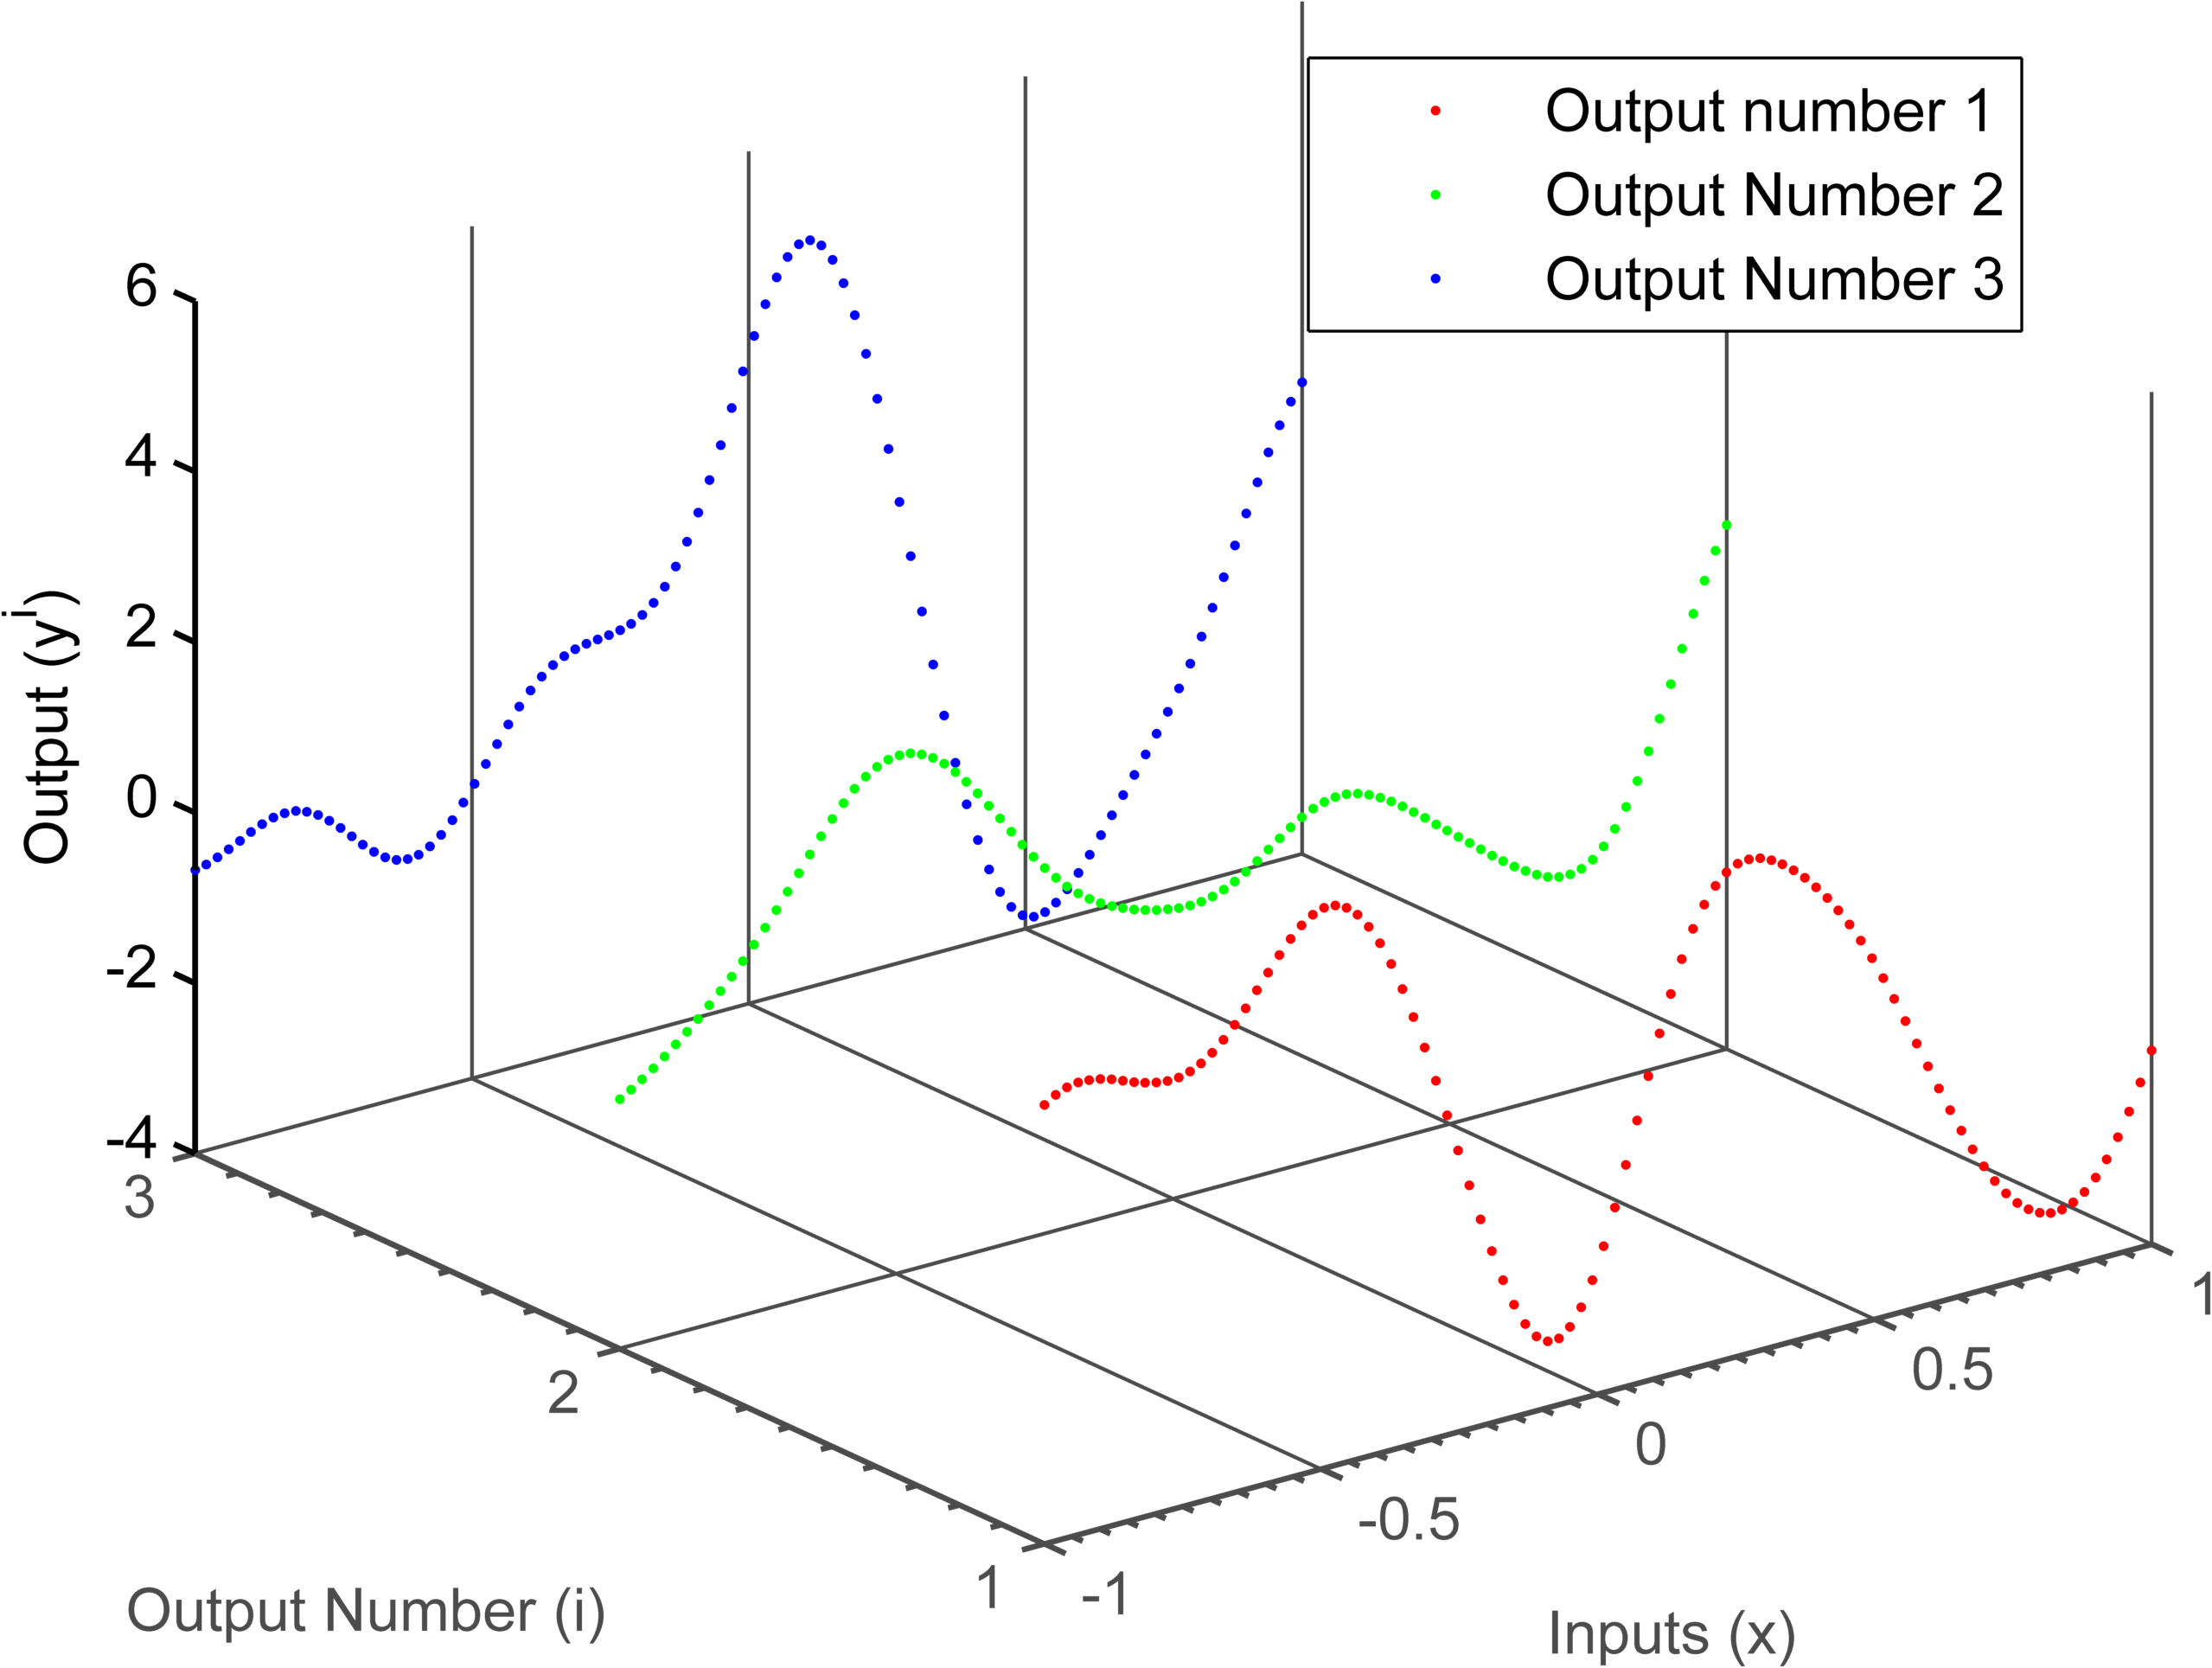
\includegraphics[width=0.45\textwidth]
        {images/part3/outputsAsAnExtraDimension}
        \label{figoutputsAsAnExtraDimension}
        \caption{The outputs can also be represented as an extra dimension.}
\end{figure}

The figure \ref{figoutputsAsAnExtraDimension} demonstrates how the different outputs can be treated as a single output coming from different dimensions. We can thus write the new input point as equation \ref{eq:modifiedInput}.

\begin{equation}\label{eq:modifiedInput}
    \VEC{x_{i}^{j}} = [x_{i1}^{j}, x_{i2}^{j}, \ldots, x_{iD_{inputs}}^{j}, j]
\end{equation}


\marginnote{\textsl{Categorical variable}}[1cm]
Note, the new input point has an extra dimension which denotes its output number. The extra dimension ($j$) is a categorical variable and hence has no measure of distance. Henceforth we define the joint output vector \(\VEC{y_{joint}}\) such that all the output values are stacked one after the other, while \(\VEC{y_{joint}} \in \mathbb{R}^{N_{joint}}\). Similarly, we define the joint input matrix as \(\myMatrix{X_{joint}}\), having one extra dimension representing the output number, such that \(\myMatrix{X_{joint}} \in \mathbb{R}^{N_{joint} \times (D_{inputs}+1)}\).  

\begin{equation}\label{eqMTGPDimension}
    \myMatrix{X_{joint}} = \begin{bmatrix}
\myMatrix{X^1}, \VEC{\mathbbm{1}_{N_{1}}} \times 1\\ 
\myMatrix{X^2}, \VEC{\mathbbm{1}_{N_{2}}} \times 2\\ 
\vdots\\ 
\myMatrix{X^{D_{outputs}}, \VEC{\mathbbm{1}_{N_{D_{outputs}}}} \times D_{outputs}}
\end{bmatrix} ; \quad 
\VEC{y_{joint}} = \begin{bmatrix}
\VEC{y^1}\\ 
\VEC{y^2}\\ 
\vdots\\ 
\VEC{y^{D_{outputs}}}
\end{bmatrix}
\end{equation}

Here, $\VEC{\mathbbm{1}_{N_{j}}}$ denotes a vector of ones to be multiplied with the `number of output'. The size of $\VEC{\mathbbm{1}_{N_{j}}}$ is $1 \times N_{j}$, $N_{j}$ is the number of data-points for the $j^{th}$ output. Since the multi-output GP can be represented as a single output GP with an extra dimension, we can use all the kernel making techniques discussed in section \ref{secMultiDimensionalKernels} to the current problem. For a case of 2 outputs we can write a zero mean GP prior for the full set of inputs and outputs $\{\myMatrix{X_{joint}}, \VEC{y_{joint}}\}$, as equation \ref{eq:mogpJointPrior}. 

\begin{equation}\label{eq:mogpJointPrior}
\begin{aligned}
       \Pr[\VEC{y_{joint}}] & = \Pr\begin{bmatrix}   \VEC{y_{joint}}(x, 1) \\ \VEC{y_{joint}}(x, 2)   \end{bmatrix} \\
& = GP\begin{bmatrix}
   \begin{pmatrix}
   0\\ 
   0
   \end{pmatrix} ,& 
   \begin{pmatrix}
    Cov(\VEC{y_{joint}}(x, 1), \VEC{y_{joint}}(x, 1))  & Cov(\VEC{y_{joint}}(x, 1), \VEC{y_{joint}}(x, 2))\\ 
    Cov(\VEC{y_{joint}}(x, 2), \VEC{y_{joint}}(x, 1))     & Cov(\VEC{y_{joint}}(x, 2), \VEC{y_{joint}}(x, 2))
   \end{pmatrix}
   \end{bmatrix}
\end{aligned}
   \end{equation}

\marginnote{\textsl{Equation \ref{eq:mogpJointPrior}}}[1cm]
Here, $Cov(\VEC{y_{joint}}(x, j), \VEC{y_{joint}}(x, j))$ is called the  auto-covariance between observations of the $j^{th}$ output, while $Cov(\VEC{y_{joint}}(x, 2), \VEC{y_{joint}}(x, 1))$ is called cross-covariance between the $2^{nd}$ and the $1^{st}$ output. Once we have the functional forms of the covariance functions, we can equivalently calculate the Gram matrix ($\myMatrix{K_{XX}}$), by replacing the values of individual input points. The upcoming sections describe different forms of covariance functions between outputs and their corresponding family of functions.

The sections \ref{simpleMultiTask} and \ref{subsecLMC} describe two simple covariance function forms when we are interested in discovering relationship between outputs, while section \ref{secMultiFidelityMTGP} describes how to impose prior information of multi-fidelity among outputs. 

\subsection{Simple Multi-task kernel}\label{simpleMultiTask}

One simple method to calculate the auto and cross-covariance functions is by simply multiplying the covariance functions for the inputs dimensions with the covariance functions for the output dimension (equation \ref{eqBonillaMTGP}), refer to \cite{bonilla2007multi} for more clarity.   

\begin{align}\label{eqBonillaMTGP}
    Cov(\VEC{y_{joint}}(x_{1}, a), \VEC{y_{joint}}(x_{2}, b)) = \FUNC{k_{output}}(a, b) \times \FUNC{k_{input}}(x_{1}, x_{2})
\end{align}

There exists one issue though, the extra dimension is a categorical variable and hence has no measure of distance, i.e. the difference between two output numbers $a$ and $b$ is not defined (equation \ref{eqBonillaMTGP}). \cite{bonilla2007multi} defined the covariance across outputs as equation \ref{eqKOutput}, this makes the matrix $\MAT{K_{output}}$ positive definite and hence a valid covariance matrix. $\FUNC{k_{output}}(a, b)$ denotes the ($a^{th}$, $b^{th}$) coordinate of the matrix $\MAT{K_{output}}$.

\begin{equation}\label{eqKOutput}
\MAT{K_{output}} = \MAT{K_{lower}}\MAT{K_{lower}}^T
\end{equation}

The hyper-parameters of above prior are the parameters of the lower triangular matrix $\MAT{K_{lower}}$, and parameters of the input  covariance function ($k_{input}(x_{1}^{a}, x_{2}^{b})$). If $\MAT{K_{output}}$ is a diagonal matrix, then there is no cross-covariance across outputs, this implies that the outputs are independent of each other. In such a kernel design there is no transfer of information between outputs \cite{bonilla2007multi, o1998markov}.

If we measure the output `$a$' at points $\myMatrix{X^1}$ and output `$b$' at not necessarily the same points $\myMatrix{X^2}$, then we can write the Gram matrix for the above prior (equation \ref{eqBonillaMTGP}) as equation \ref{eqGramMatrixSimpleMultiTask}.

\begin{equation}\label{eqGramMatrixSimpleMultiTask}
   \MAT{K_{XX}} =  \begin{bmatrix} k_{output}(a, a) \cdot \myMatrix{K}_{input}(\myMatrix{X^1}, \myMatrix{X^1}) & 
k_{output}(a, b) \cdot \myMatrix{K}_{input}(\myMatrix{X^1}, \myMatrix{X^2}) \\ 
k_{output}(b, a) \cdot \myMatrix{K}_{input}(\myMatrix{X^2}, \myMatrix{X^1}) &
k_{output}(b, b) \cdot \myMatrix{K}_{input}(\myMatrix{X^2}, \myMatrix{X^2}) 
\end{bmatrix}
\end{equation}


Here, `$\cdot$' denotes the multiplication between a scalar and a matrix. 

\begin{figure}[!ht]
  \centering
    \subfigure[{Five randomly drawn functions for output number 1, using the MTGP kernel proposed by \cite{bonilla2007multi}}]
  {
        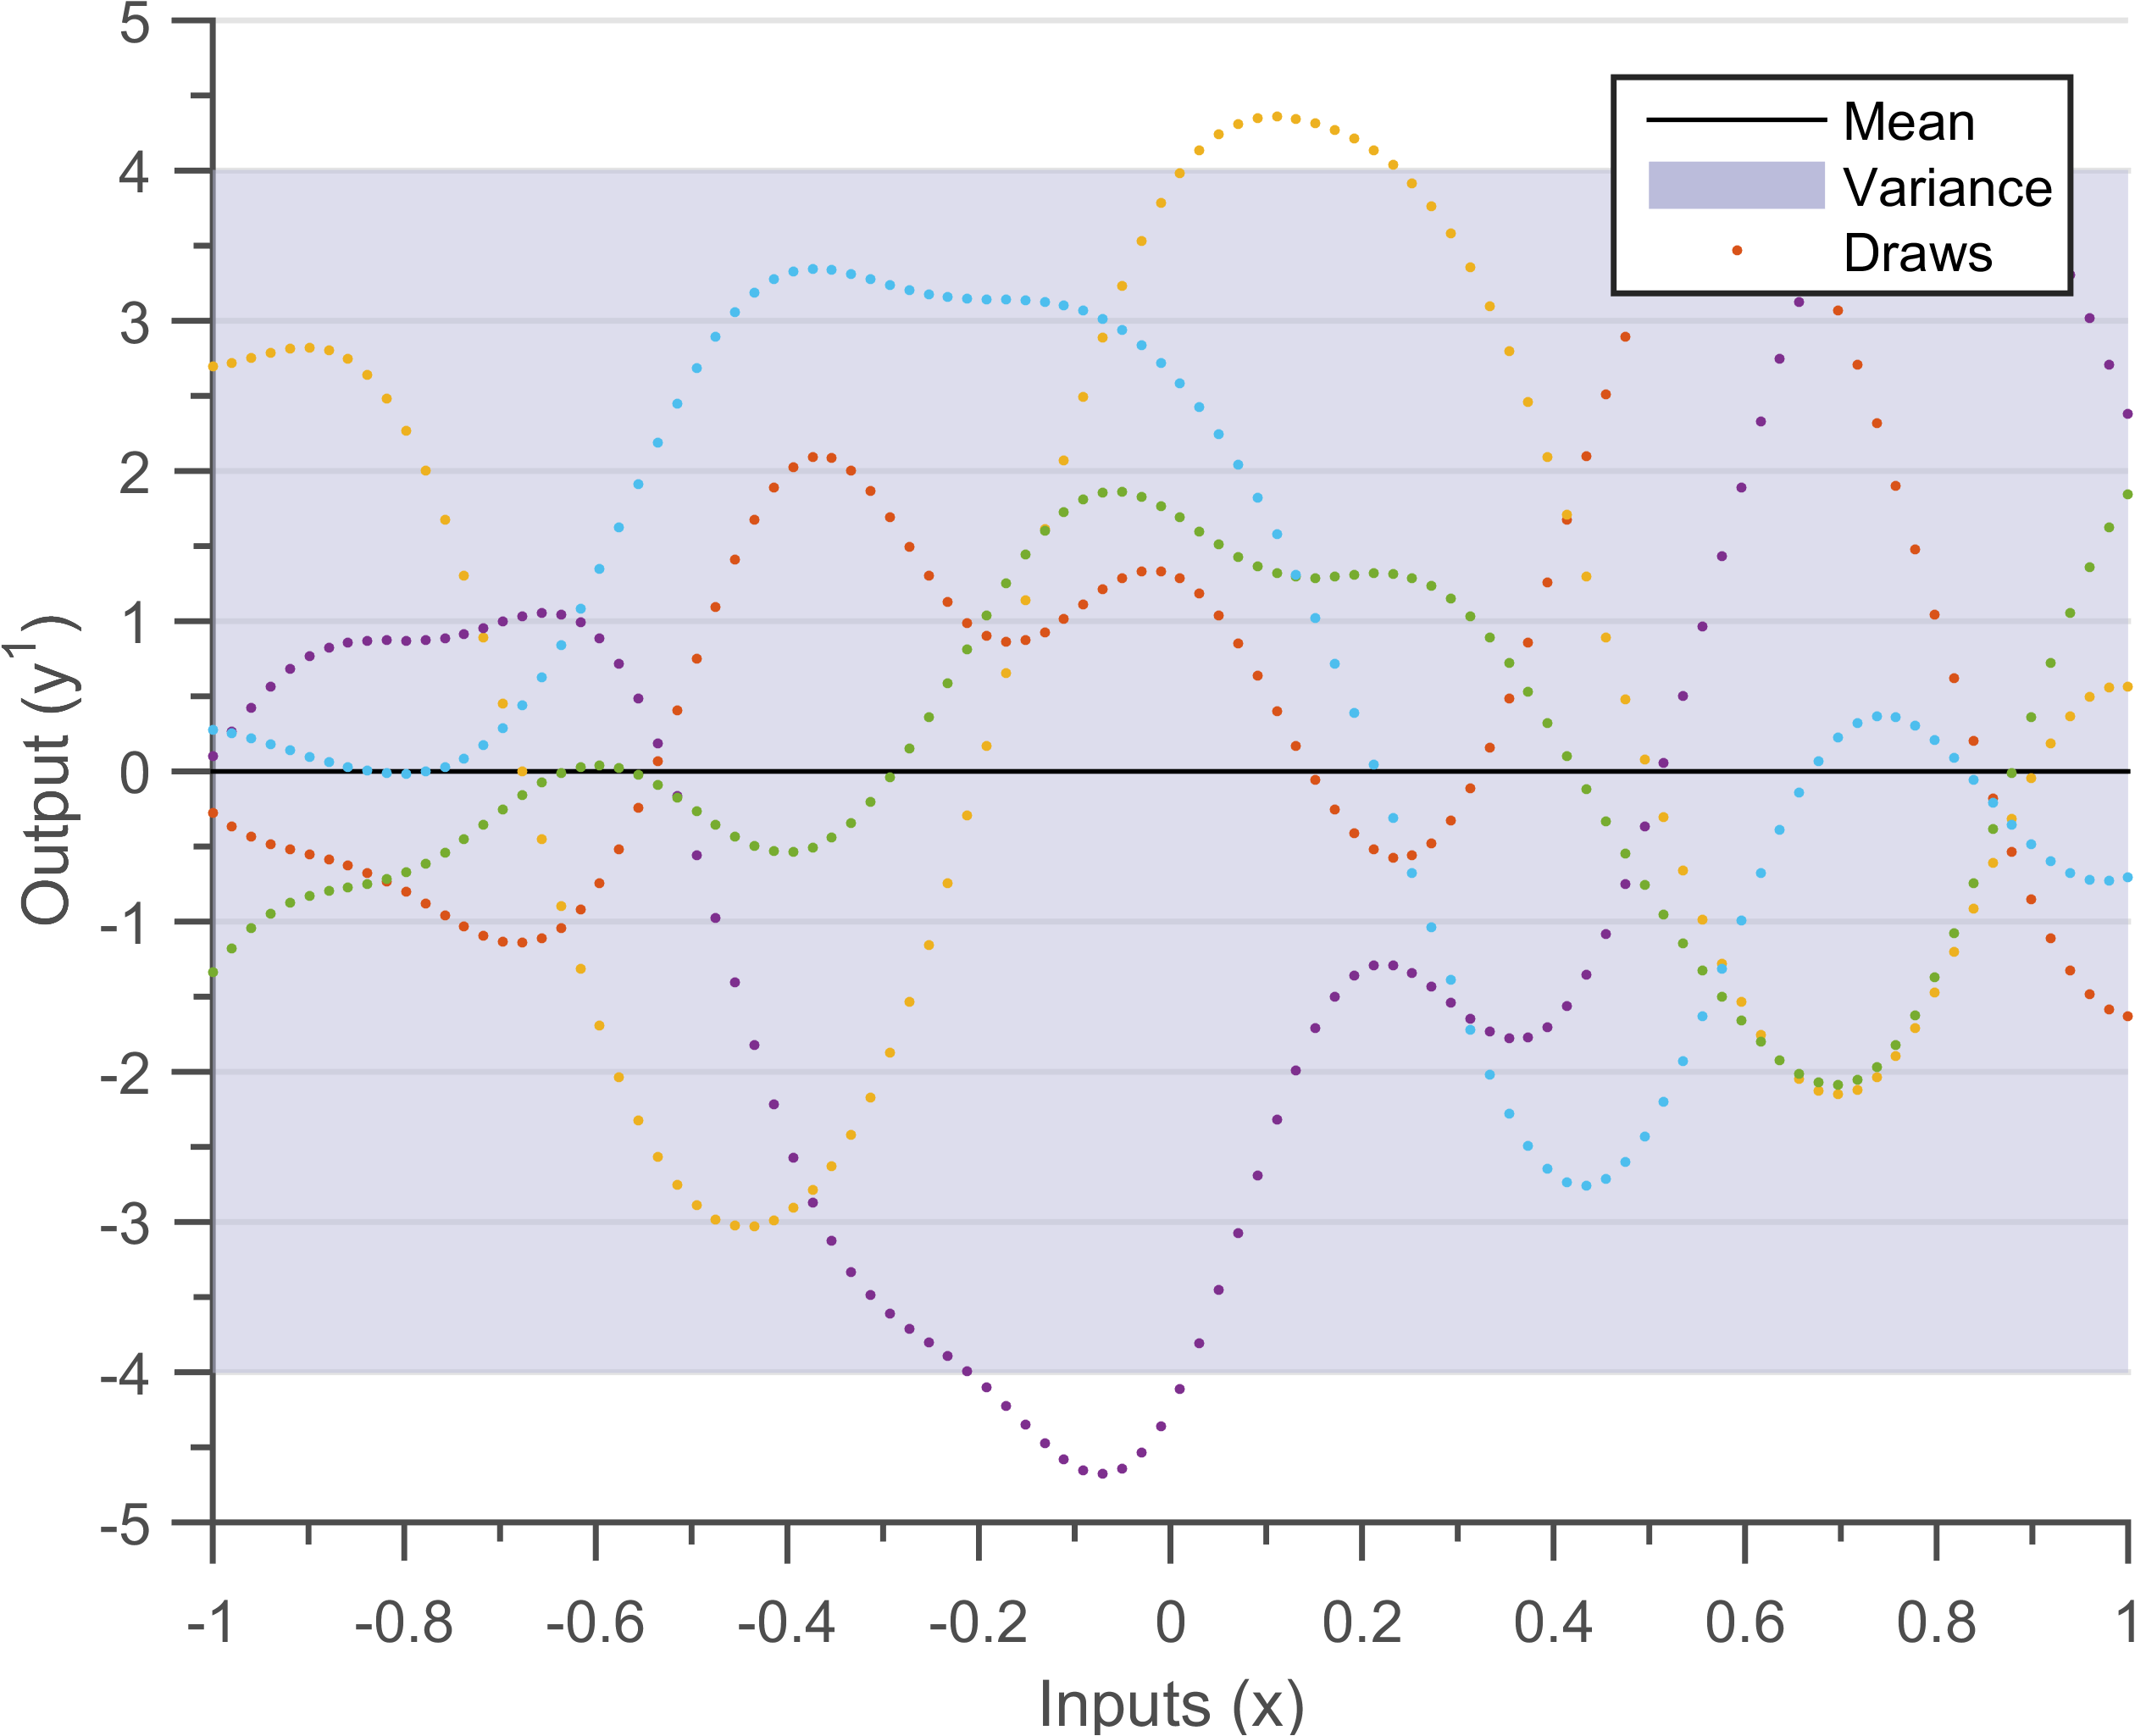
\includegraphics[width=0.45\textwidth]
        {images/part3/drawsBonillaKernelOutput1}
        \label{subFigdrawsBonillaKernelOutput1}
  }\quad
\subfigure[{Five randomly drawn functions for output number 2, using the MTGP kernel proposed by \cite{bonilla2007multi}}]
  {
        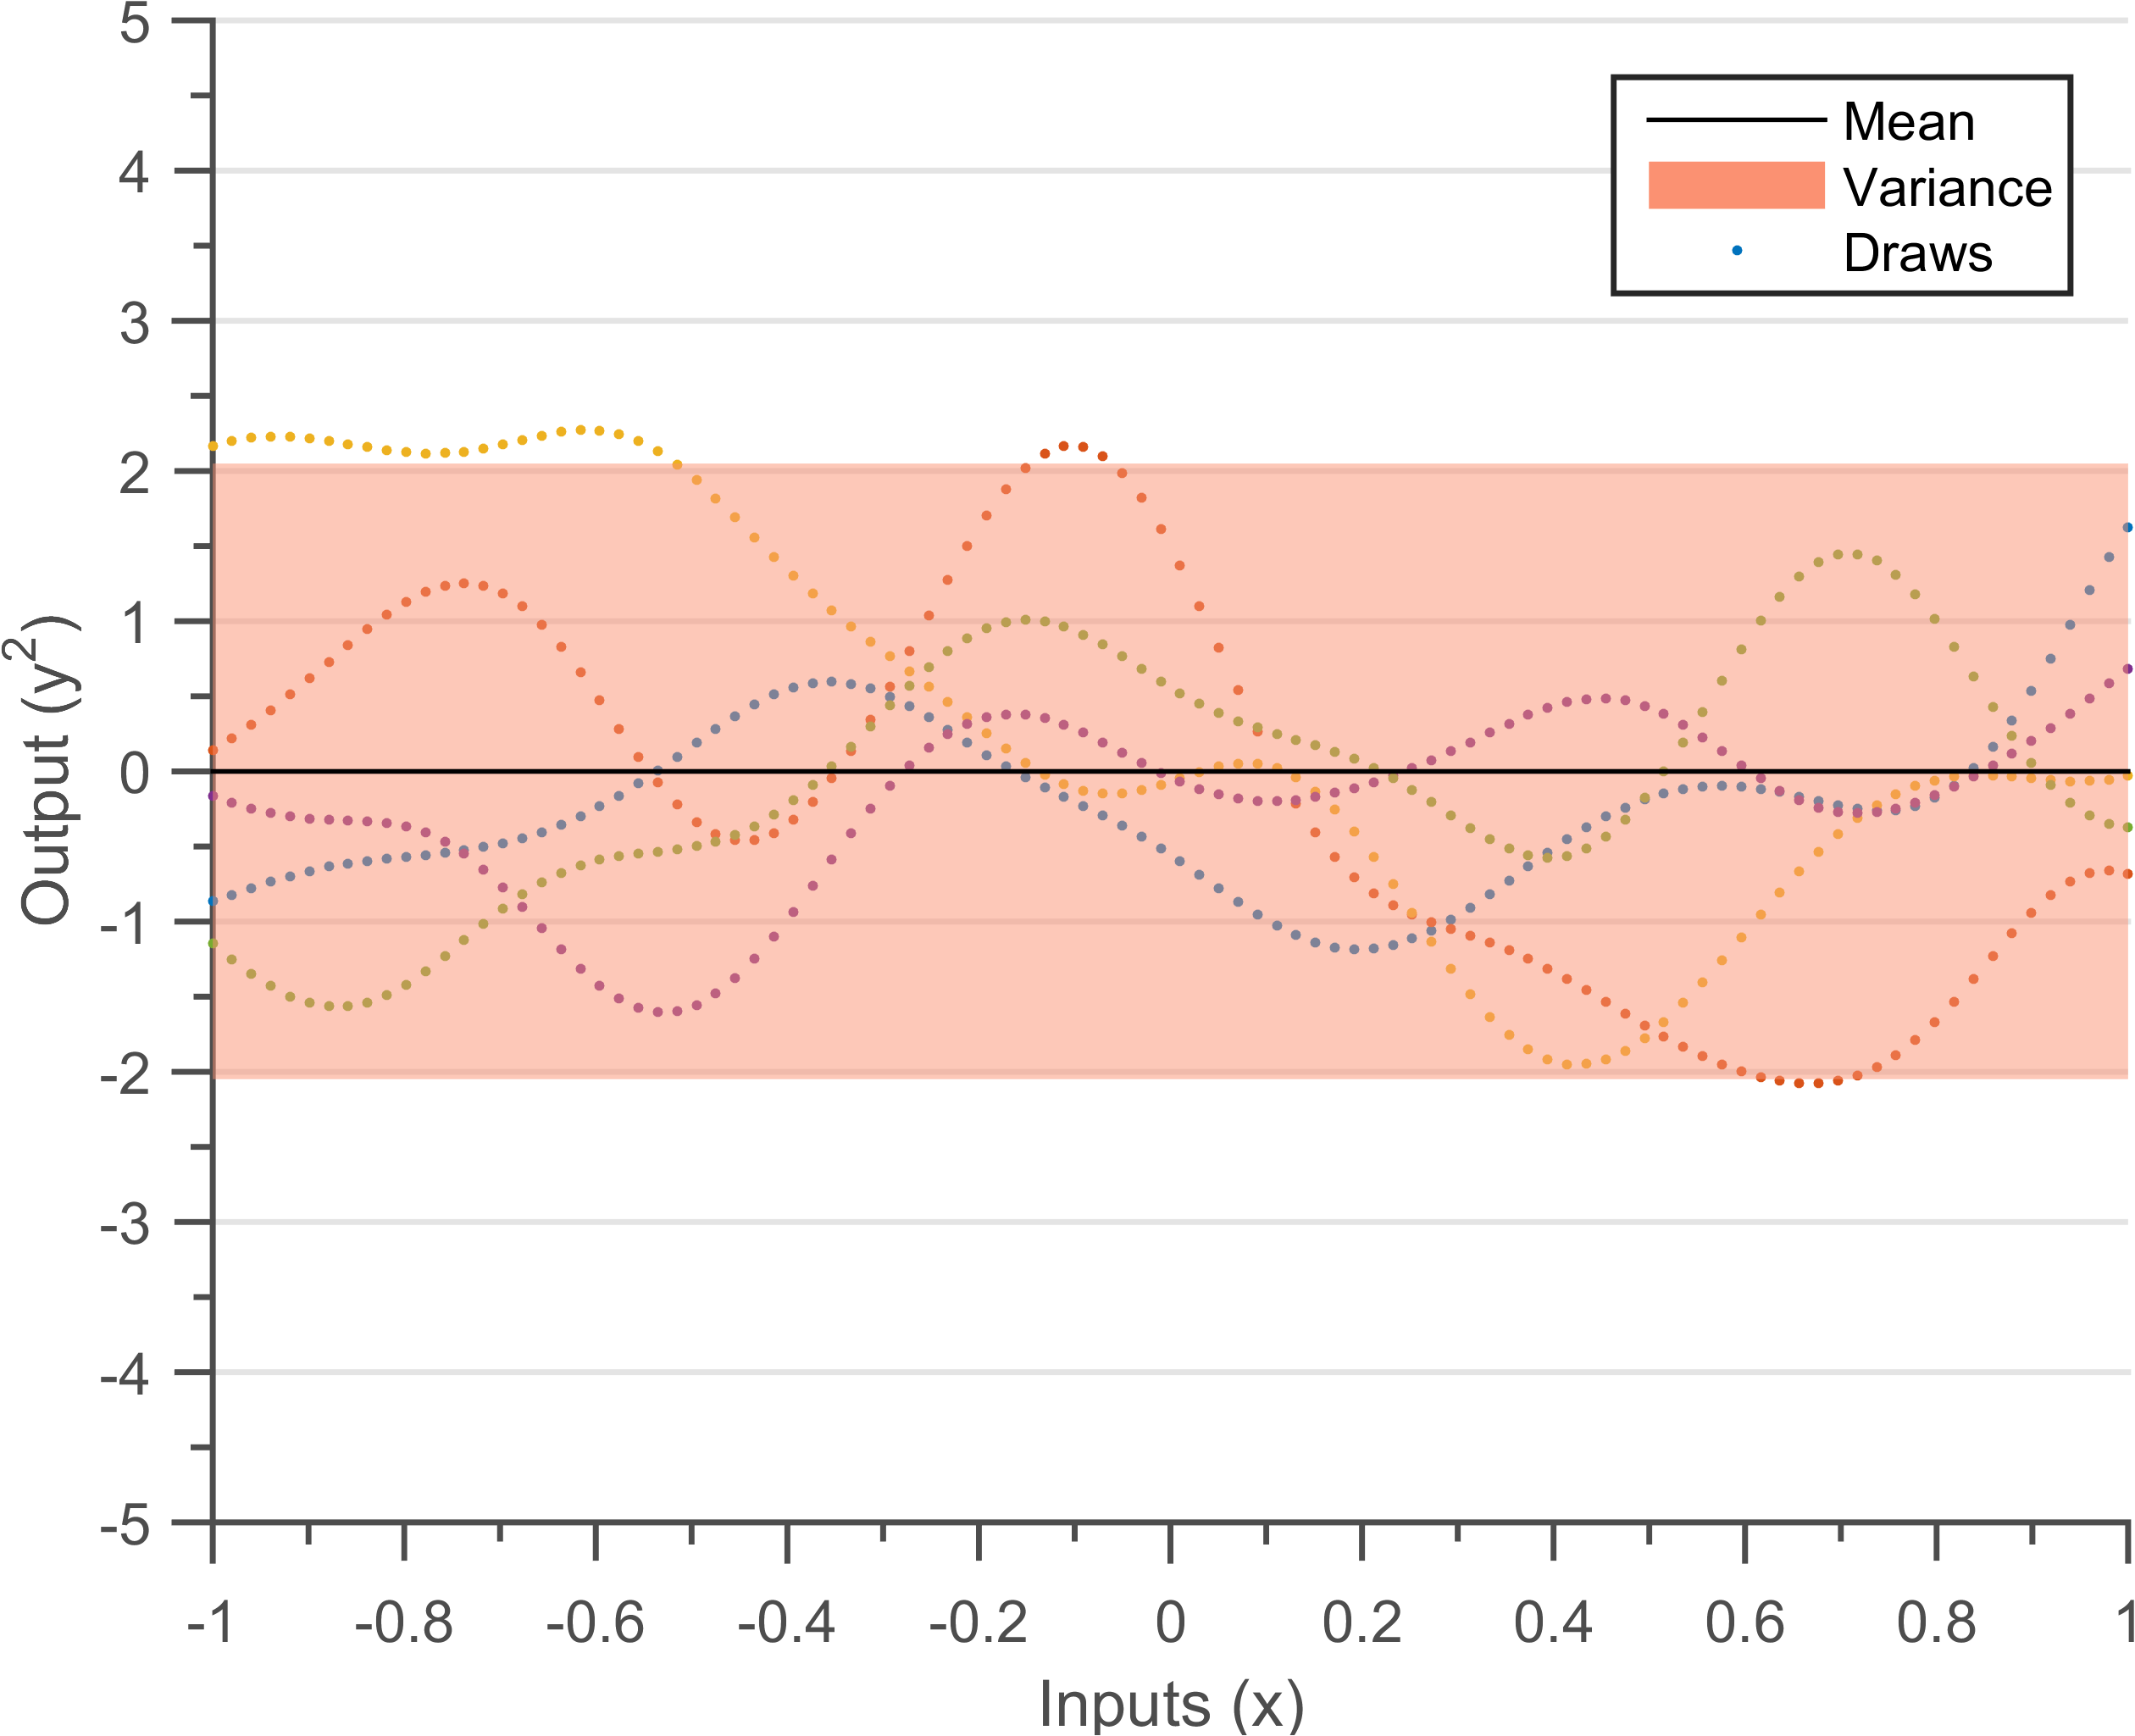
\includegraphics[width=0.45\textwidth]
        {images/part3/drawsBonillaKernelOutput2}
        \label{subFigdrawsBonillaKernelOutput2}
  }\quad

       \caption{Joint draws from a simple multi-task kernel function between outputs $y^{1}$ and $y^{2}$. The matrix  $\MAT{K_{output}} = [4 , 0.2; 0.2 , 1]$ while the covariance function between inputs $\FUNC{k_{input}}(x_{1}, x_{2})$ is a SE kernel with hyper-parameters $(\theta = [1, 0.2])$. The solid black line defines the mean function, shaded region defines 95\% confidence interval (2$\sigma$) distance away from the mean. The dashed lines represent five functions drawn at random from a GP prior. We can observe that figure \ref{subFigdrawsLCMKernel} varies faster when compared to figure \ref{subFigdrawsBonillaKernel} due to smaller length scale hyper-parameter in one of the latent functions.}
       \label{subFigdrawsBonillaKernel}
\end{figure}

Figure \ref{subFigdrawsBonillaKernel} is a joint draw from such a kernel function between outputs $y^{1}$ and $y^{2}$. The matrix $\MAT{K_{output}} = \bigl( \begin{smallmatrix} 4 & 0.2\\ 0.2 & 1\end{smallmatrix}\bigr)$ while the covariance function between inputs $\FUNC{k_{input}}(x_{1}, x_{2})$ is a SE kernel with hyper-parameters $(\theta = [1, 0.2])$. We can observe that the variance of output $y^{1}$ is twice that of output $y^{2}$, this is because $\sqrt{k_{output}(1, 1)/k_{output}(2, 2)} = 2$.


\subsection{Linear Model of Coregionalization}\label{subsecLMC}
The next method considers the output variables as a linear combination of independent latent GPs. It is called the Linear Model of Coregionalization in kriging literature \cite{goovaerts1997geostatistics} or Semiparametric Latent Factor Model in MTGP literature \cite{seeger2005semiparametric}. Latent GPs are random variables which are not directly observed. 

Suppose we have a set of $L$ latent GPs $U(x) = \{u^{1}(x), u^2(x), \ldots, u^{L}(x)\}$, where $u^{i}(x)$ is a GP with covariance $k_{u}^{i}(x_{1}, x_{2})$. Any linear combination of $u^{i}(x) \quad \forall i \in L$ is a viable GP (section \ref{subsecStructureKernelsAddingKernels}), therefore we can define the GP of output $y^{j}$ as equation \ref{eqLinearCombo}. 

\begin{equation}\label{eqLinearCombo}
y^{j}(x) = \sum_{i=1}^{L} \alpha^{ij}u^{i}(x)
\end{equation}

The covariance function can thus be written as equation \ref{eqCovarianceLMC}.

\begin{equation}\label{eqCovarianceLMC} 
 \begin{aligned}
Cov(\VEC{y_{joint}}(x_{1}, a), \VEC{y_{joint}}(x_{2}, b)) & = Cov(\sum_{i=1}^{L} \alpha^{ia}u^{i}(x_{1}), \sum_{i=1}^{L} \alpha^{ib}u^{i}(x_{2})) \\ 
& = \sum_{i=1}^{L} \alpha^{ia}\alpha^{ib} Cov(u^{i}(x_{1}), u^{i}(x_{2})) \\ 
& = \sum_{i=1}^{L} \alpha^{ia}\alpha^{ib}k_{u}^{i}(x_{1}, x_{2}) \\ 
& = \sum_{i=1}^{L} \MAT{K_{output}^{i}}(a, b) \cdot k_{u}^{i}(x_{1}, x_{2})
 \end{aligned}
\end{equation}

The covariance between the output dimension \MAT{K_{output}^{i}} is also called the coregionalization matrix, and is of size $D_{outputs} \times D_{outputs}$. It can be written as equation \ref{eqCovarianceAcrossOutputs}, making it a positive definite matrix \cite{mercer1909functions}.

\begin{equation}\label{eqCovarianceAcrossOutputs}
\MAT{K_{output}^{i}} = \begin{bmatrix}
\alpha^{i1}\\ 
\alpha^{i2}\\ 
\vdots\\ 
\alpha^{iD_{outputs}}
\end{bmatrix} \cdot \begin{bmatrix}
\alpha^{i1} & \alpha^{i2} & \ldots & \alpha^{iD_{outputs}}
\end{bmatrix}
\end{equation}

Note, when $L = 1$ and $D_{outputs} > 1$ the Linear Model of Coregionalization is equivalent to the model proposed by \cite{bonilla2007multi}. While, when $L > 1$ and $D_{outputs} = 1$ the Linear Model of Coregionalization model resembles an additive covariance of $T$ individual covariances (section \ref{subsecStructureKernelsAddingKernels}).

Figure \ref{subFigdrawsLCMKernel} shows 3 joint draws from a `Linear Model of Coregionalization' kernel function between outputs $y^{1}$ and $y^{2}$. We use two latent functions for this figure; the kernels between output dimensions are $\MAT{K_{output}}^{1} = \bigl( \begin{smallmatrix} 4 & 0.2\\ 0.2 & 1\end{smallmatrix}\bigr)$ and $\MAT{K_{output}}^{2} = \bigl( \begin{smallmatrix} 1 & 0.2\\ 0.2 & 1\end{smallmatrix}\bigr)$, while the covariance function between inputs are SE kernel with hyper-parameters $(\theta = [1, 0.2])$ for the first latent process and $(\theta = [1, 0.1])$ for the second latent process. The length-scale of the functions is determined by the smallest length-scale of the latent processes.
\marginnote{\textsl{Figure \ref{subFigdrawsLCMKernel}}}[-1cm]

\begin{figure}[!ht]
  \centering
    \subfigure[{Five randomly drawn functions for output number 1, using the MTGP kernel proposed by Linear Model of Coregionalization}]
  {
        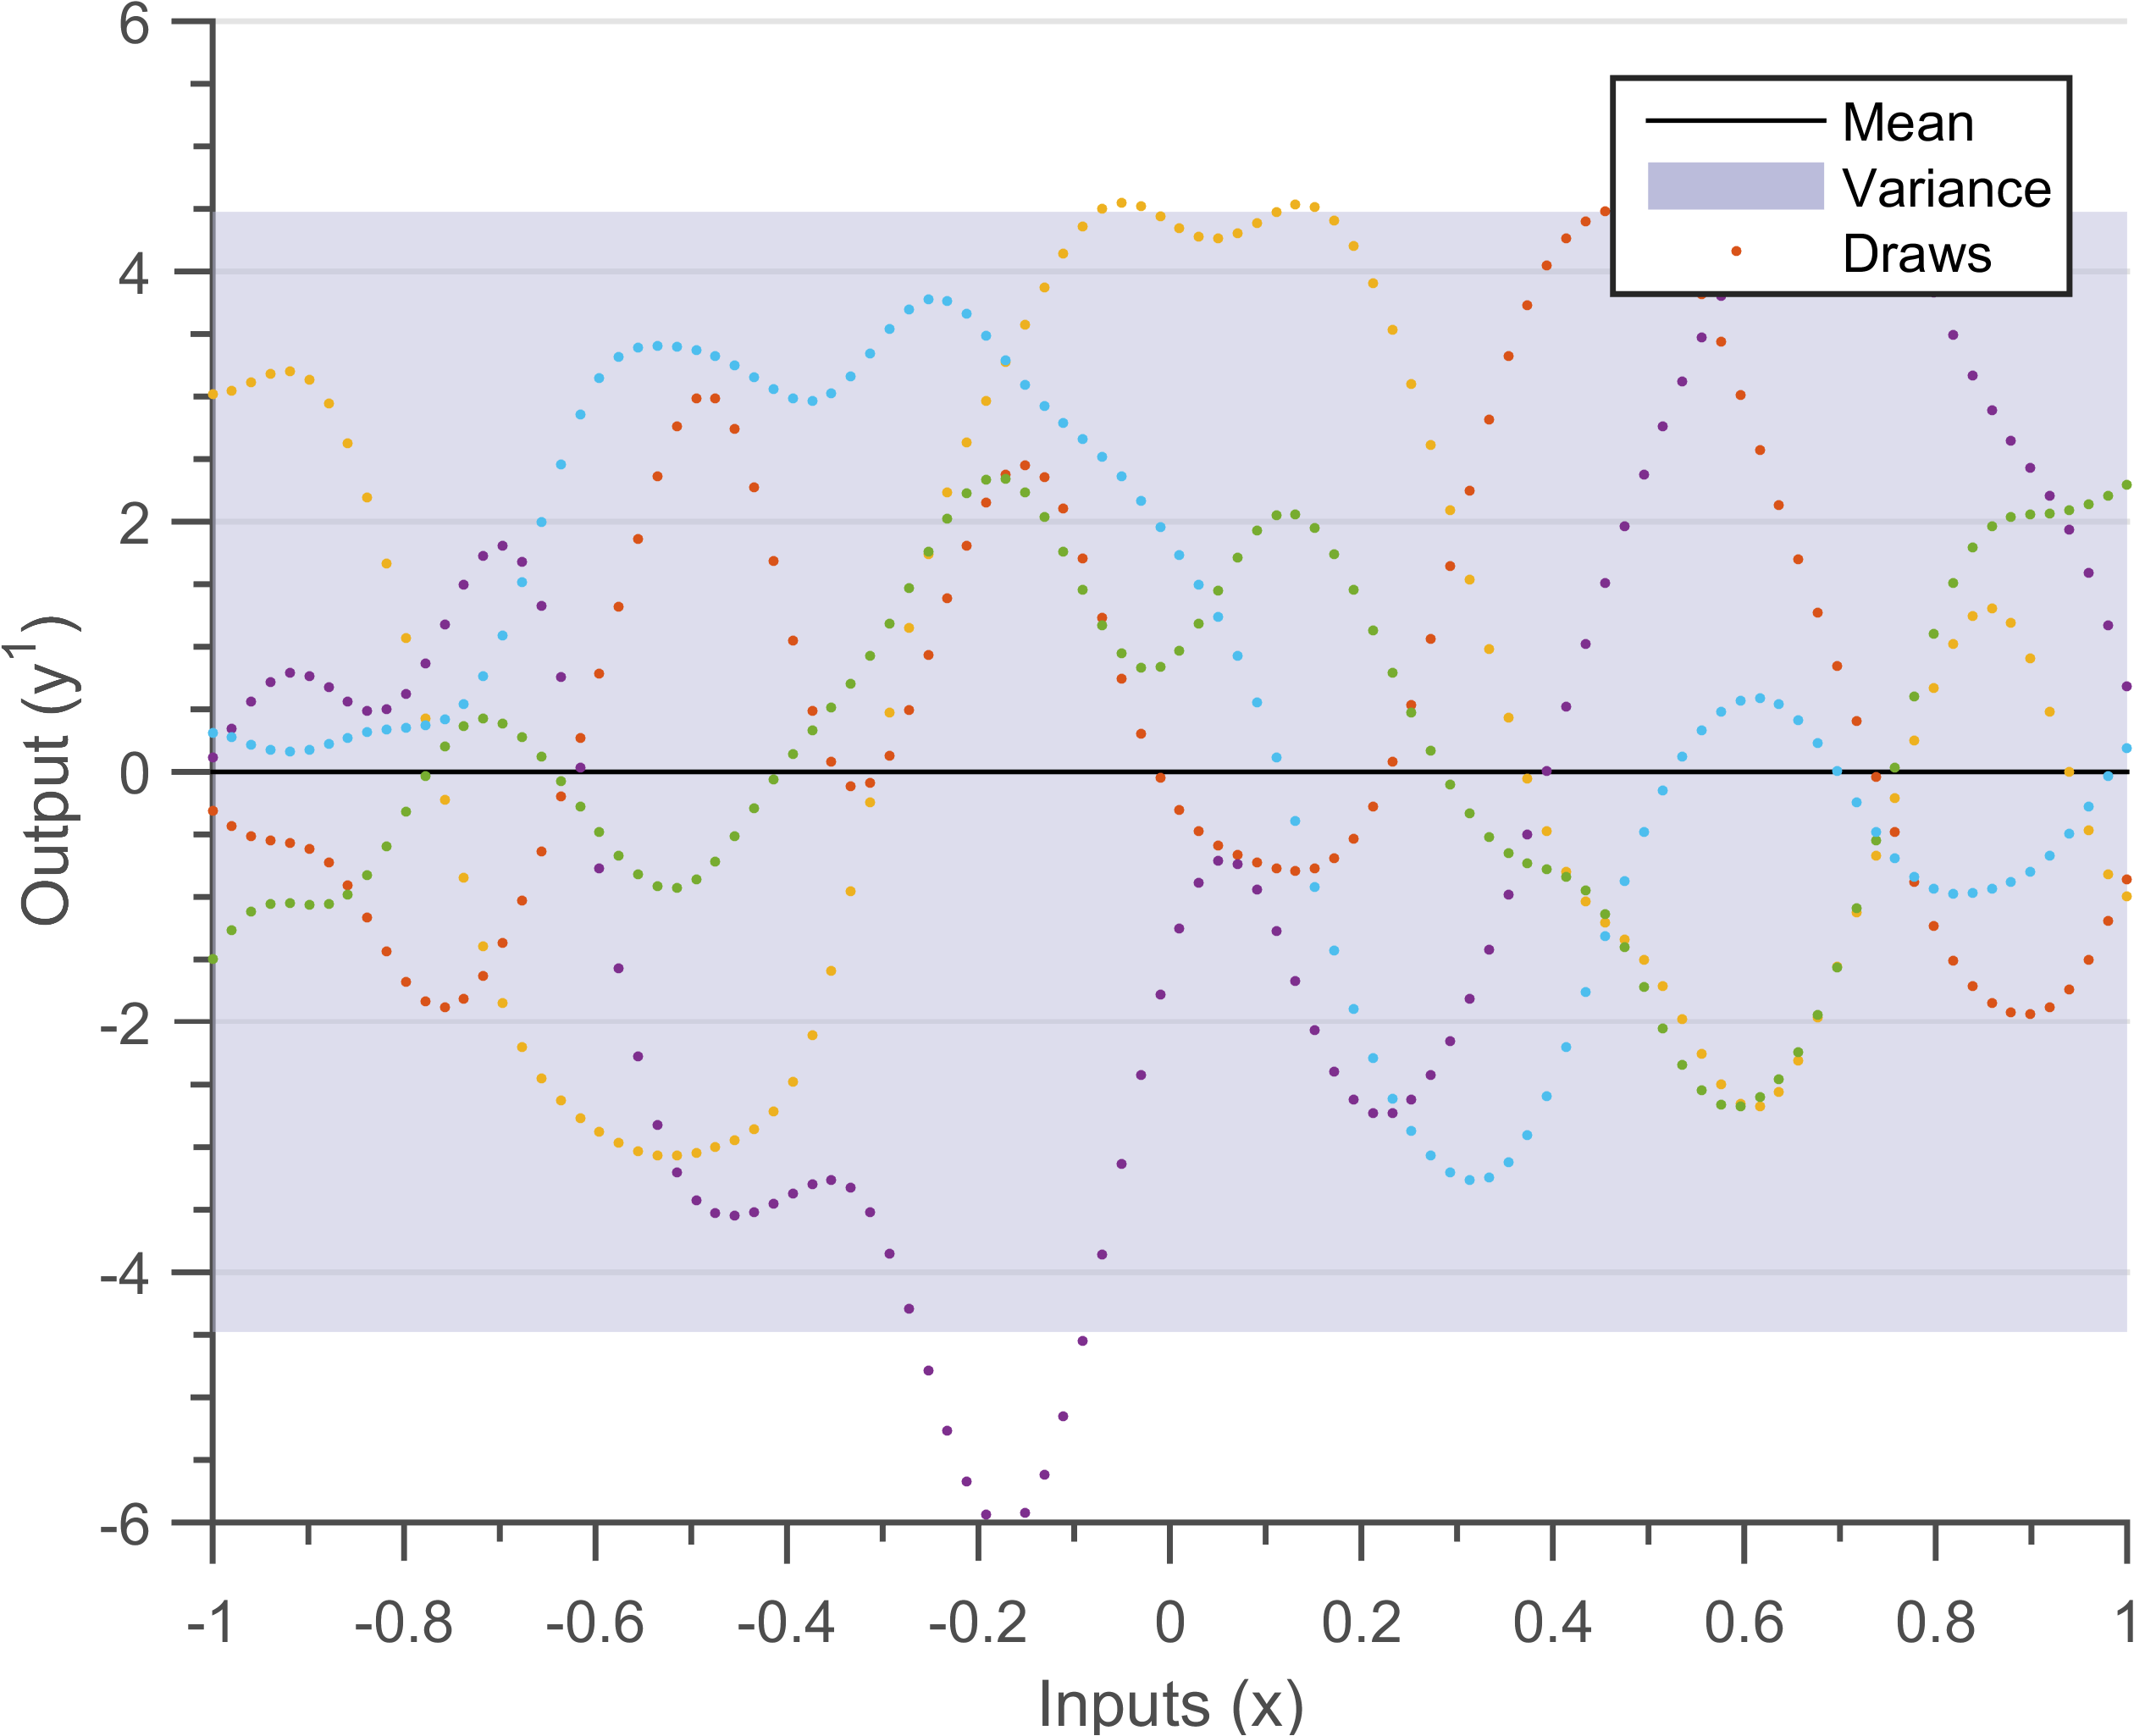
\includegraphics[width=0.45\textwidth]
        {images/part3/drawsLCMKernelOutput1}
        \label{subFigdrawsLCMKernelOutput1}
  }\quad
\subfigure[{Five randomly drawn functions for output number 2, using the MTGP kernel proposed by Linear Model of Coregionalization }]
  {
        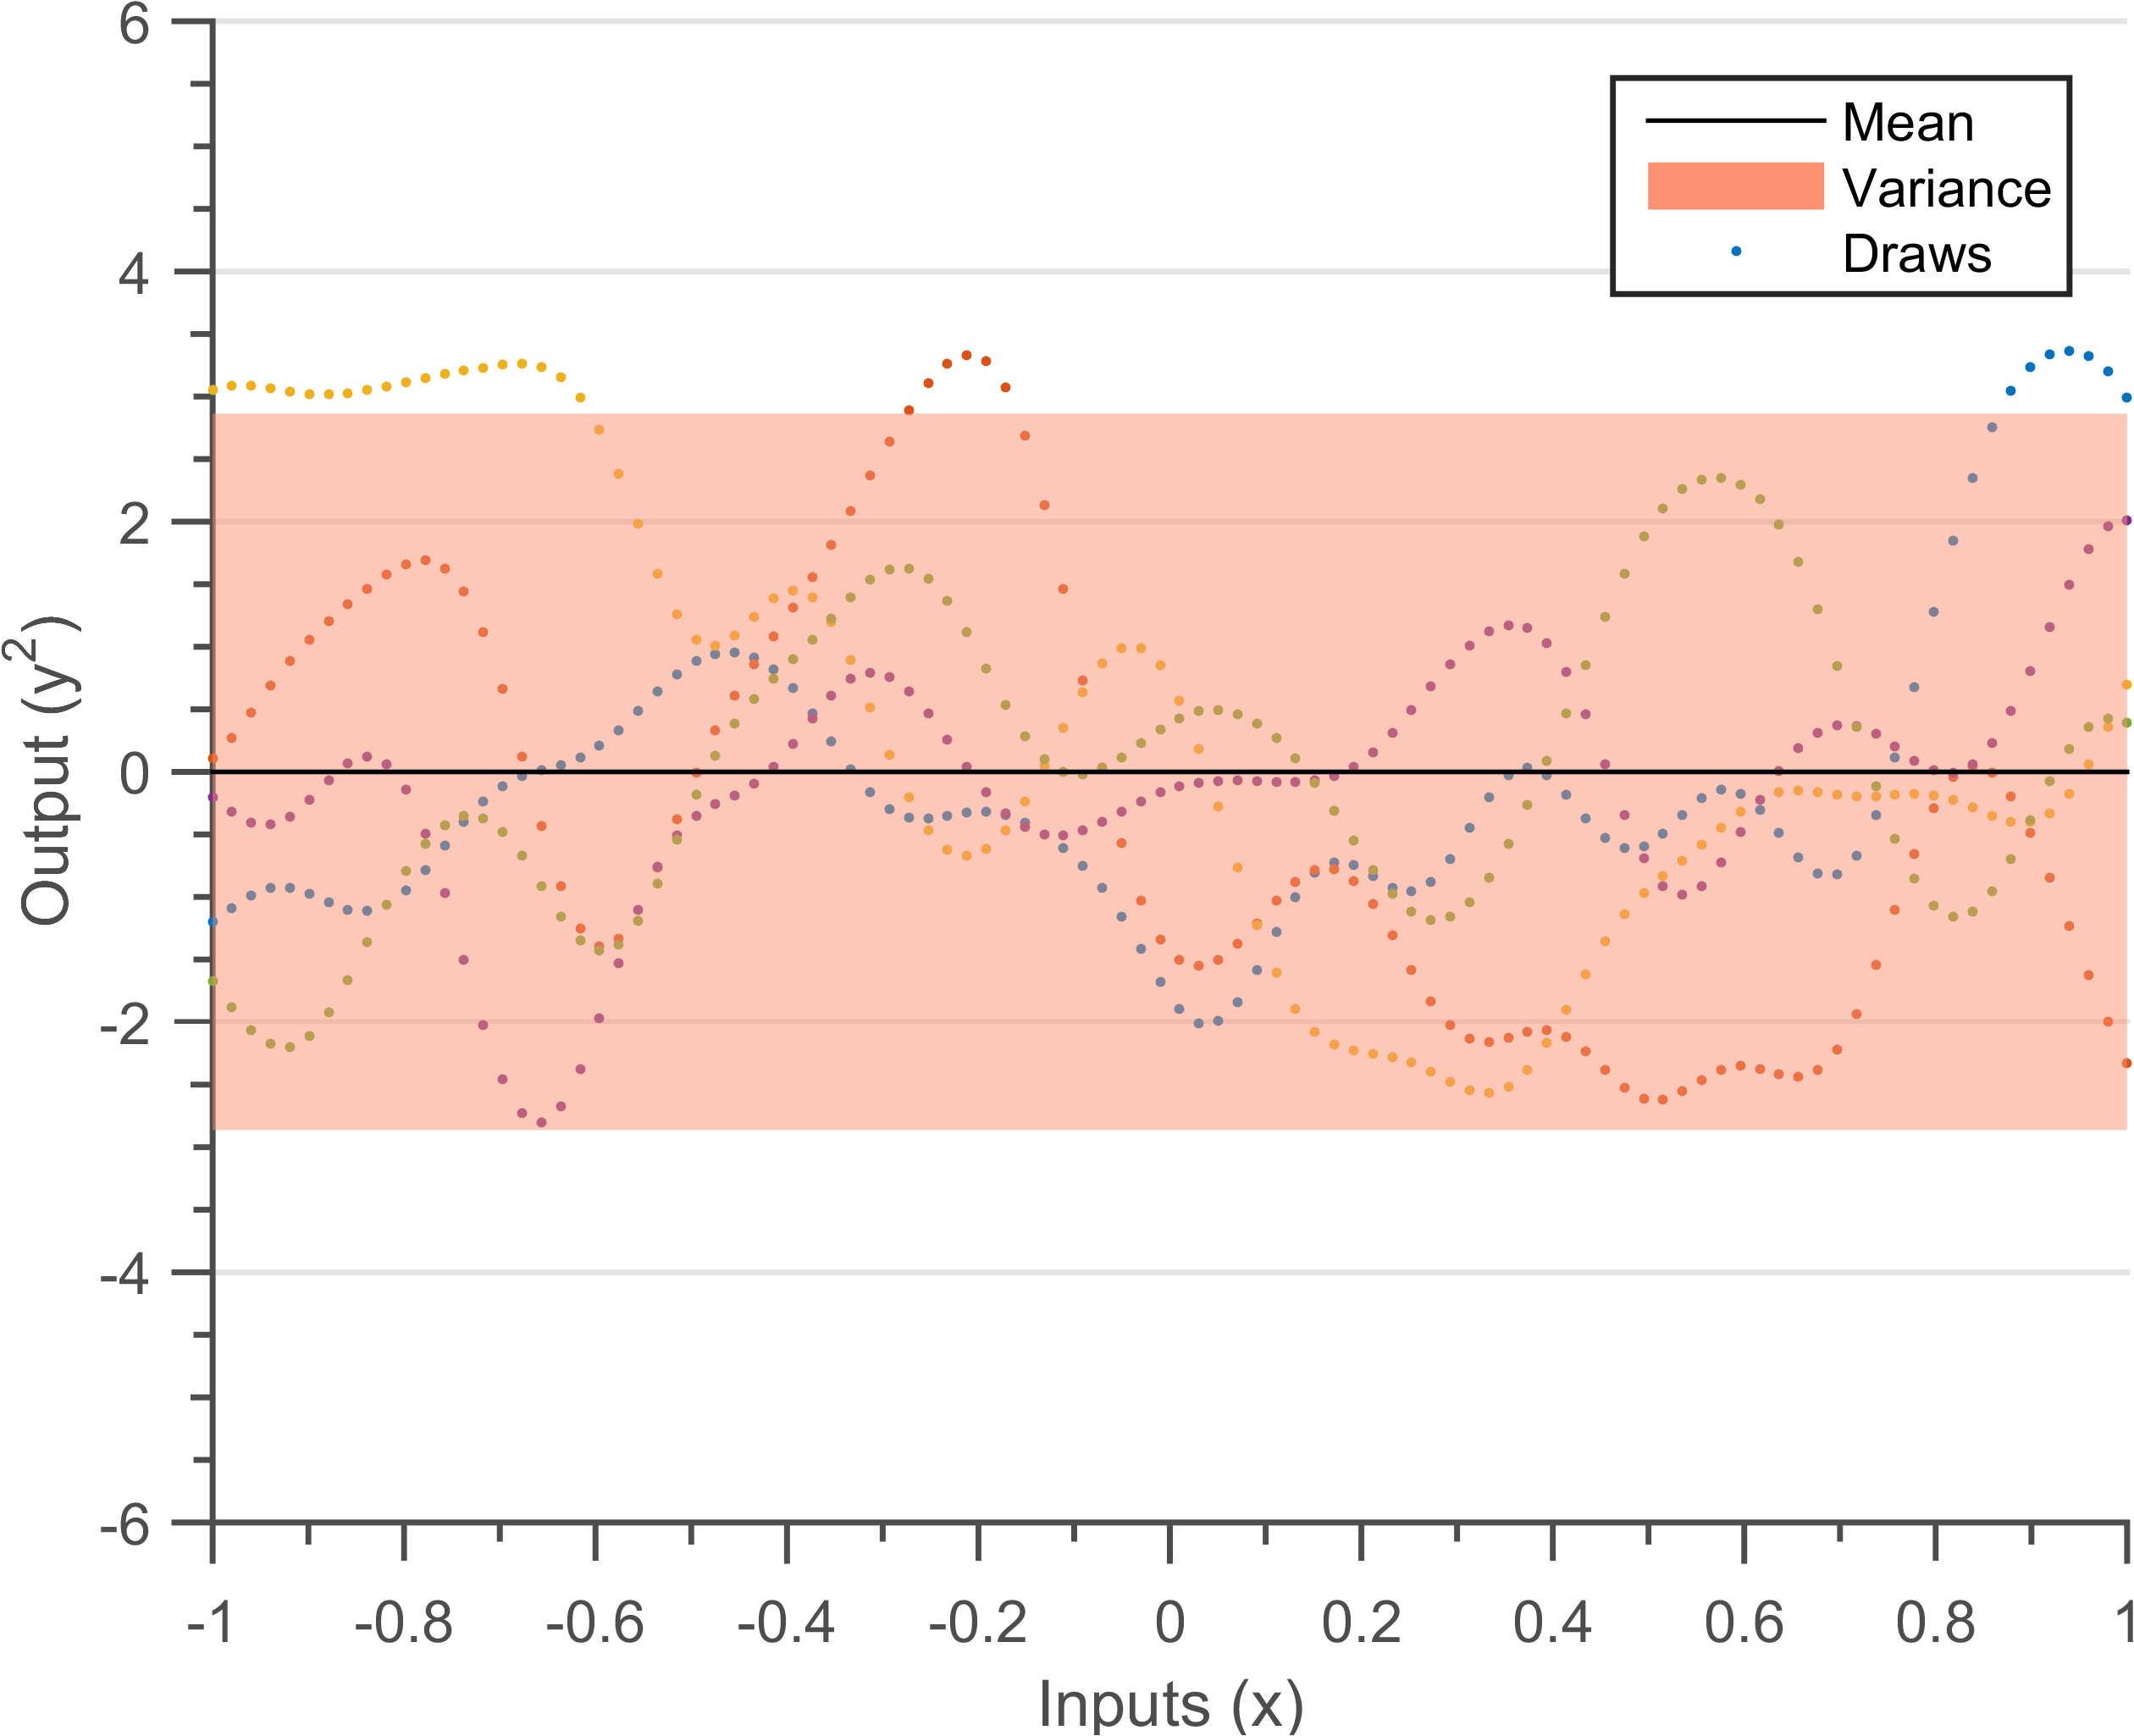
\includegraphics[width=0.45\textwidth]
        {images/part3/drawsLCMKernelOutput2}
        \label{drawsLCMKernelOutput2}
  }\quad

       \caption{Joint draws from a `Linear Model of Coregionalization' kernel function between outputs $y^{1}$ and $y^{2}$. We use two latent functions for figure; the kernels between output dimensions are $k_{output}^{1} = [4, 0.2; 0.2, 1]$ and $k_{output}^{2} = [1, 0.2; 0.2, 1]$, while the covariance function between inputs are SE kernel with hyper-parameters $(\theta = [1, 0.2])$ for the first latent process and $(\theta = [1, 0.1])$ for the second latent process. The solid black line defines the mean function, shaded region defines 95\% confidence interval (2$\sigma$) distance away from the mean. The dashed lines represent five functions drawn at random from a GP prior. We can observe that figure \ref{subFigdrawsLCMKernel} varies faster when compared to figure \ref{subFigdrawsBonillaKernel} due to smaller length scale hyper-parameter in one of the latent functions.}
       \label{subFigdrawsLCMKernel}
\end{figure}

\subsection{Multi-fidelity GP}\label{secMultiFidelityMTGP}
Simulation models in engineering design often come with different orders of accuracy or fidelity. The increase in accuracy is generally associated to an increase in cost. This is because capturing the higher order effects means either more non-linear models or finer meshes. This creates an opportunity to reduce the overall cost of accurate predictions by reducing the number of runs of the costly, high-fidelity computation and launching several low-fidelity computations. We can treat the low-fidelity and high-fidelity predictions as cases with multiple outputs. The prior information that we have here is that one output is more precise than another. 

\cite{kennedy2000predicting, o1998markov} proposed the first Cokriging model for multi-fidelity calculations. This method has been used extensively to make cheaper surrogate models and perform cheap optimization of a costly code \cite{forrester2007multi, march2012provably}. We will describe the methods proposed by \cite{o1998markov} in this section. 

Suppose we have $D_{outputs}$ simulation models $y^{i}(x)$  $\forall$ $ i \in D_{outputs}$, ordered with increasing levels of accuracy. Since these are simulations of a computer code there is no noise in the outputs. \cite{o1998markov} used the Markov property (equation \ref{eqMarkovProperty}) between a higher fidelity code $y^{i}(x)$ and lower fidelity code $y^{i-1}(x')$ for all $x \neq x'$. This assumption means that no further information about $y^{i}(x)$ can be extracted from lower level models if we have access to simulation results at the same input point. 

\begin{equation}\label{eqMarkovProperty}
         Cov(y^{i}(x), y^{i-1}(x') \mid y^{i-1}(x)) = 0
\end{equation}

\marginnote{\textsl{Linearly separable}}[1cm]
The Markov property assumption means that if there are two subsequent fidelity models $y^{i}(x)$ and $y^{i-1}(x)$. Then the high-fidelity model ($y^{i}(x)$) can be represented as a linear combination of the low-fidelity model ($y^{i-1}(x)$) and a model that represents the difference between the two ($\delta^{i}(x)$), thereby linearly seperating the effects of the two models. It can be expressed equivalently as the set of equations below. 

\begin{align}
  & y^{i}(x) = r^{i-1}(x)y^{i-1}(x) + \delta^{i}(x) \\
  & y^{i-1}(x) \perp \delta^{i}(x)
\end{align}

Here, $r^{i-1}(x)$ is a continuous function in $x \in \mathbb{R}$, $\perp$ signifies independence between two GPs ($Cov(y^{i-1}(x), \delta^{i}(x)) = 0$). If we have 2 sets of simulation results with varying fidelity $y^{2}(x)$ more accurate than $y^{1}(x)$, the above model gives rise to the following joint-covariance structure.

\begin{equation}\label{eqJointCovarianceMultiFidelity}
         \begin{aligned}
           \myMatrix{K_{XX}}   & = \begin{bmatrix} k^{1}(x^{1}, x^{1}) & r(x^{1})k^{1}(x^{1}, x^{2})   \\
           r(x^{2})k^{1}(x^{2}, x^{1}) & r(x^{2})^2k^{1}(x^{2}, x^{2}) + k^{\delta}(x^{2}, x^{2}) \end{bmatrix} \\ 
           & = \begin{bmatrix} k^{1}(x^{1}, x^{1}) & r(x^{2})k^{1}(x^{1}, x^{2})   \\ r(x^{1})k^{1}(x^{2}, x^{1}) & r(x^{2})^2k^{1}(x^{2}, x^{2}) \end{bmatrix} 
           +  
\begin{bmatrix} 0 & 0 \\ 0 & k^{\delta}(x^{2}, x^{2}) \end{bmatrix} 
         \end{aligned}
\end{equation}

Here, $x^{1}$ are the input points for simulation $y^{1}$, and $x^{2}$ are the simulation points for output $y^{2}$, $k^{1}(x^{1}, x^{2})$ is the covariance function for output $y^{1}$. $k^{1}$ represents the covariance function for output $y^1$, $k^{2}$ represents the covariance function for output $y^2$ and $k^{\delta}$ represents the covariance function for difference between the two models $\delta$. \cite{kennedy2000predicting} have used a constant function for the value of $r(x)$ and an SE kernel for the covariances $k^{1}(x, x')$ and $k^{\delta}(x, x')$. 

The model of multi-fidelity GPs in equation \ref{eqJointCovarianceMultiFidelity} is equivalent to a `Linear Model of Coregionalization' model with two latent processes. The fist process has $\MAT{K_{output}}^{1} = \bigl( \begin{smallmatrix} 1 & r\\ r & r^2\end{smallmatrix}\bigr)$ as covariance between outputs and $\FUNC{k_{inputs}^1 = k^1}$ as the covariance between inputs, while the second process has $\MAT{K_{output}}^{2} = \bigl( \begin{smallmatrix} 0 & 0\\ 0 & 1\end{smallmatrix}\bigr)$ as the covariance between outputs and $\FUNC{k_{inputs}^2 = k^\delta}$ as the covariance between inputs. We have thus linearly seperated the effects of both the models, such that the difference between the two is captured by the $k^{\delta}(x, x')$ covariance function.

\marginnote{\textsl{Recursive model}}[1cm]
Multi-fidelity GPs are expensive due to the cost of calculating the precision matrix. \cite{le2013multi} proposed a recursive model for performing multi-fidelity, this model performs the learning for individual computer codes thereby breaking the Gram matrix into smaller sizes and reducing the computational complexity. They also extend the Cokriging model to several number of multiple outputs.

\subsection{Posterior distribution}\label{subsecPosteriorDistribution}
For simplicity let us take the case of two outputs \(y^{1}\) and \(y^{2}\). Suppose we measure the two outputs with some error ($\epsilon_{n1}$ and $\epsilon_{n2}$), while the true physical process is defined by latent variables (\(f^{1}\) and \(f^{2}\)). Then the relation between the output function, measurement error, and true physical process can be written as follows. 

\begin{align} \label{eq:relationOutputLatent}
y^{1} & = f^{1} + \epsilon_{n1} \\
y^{2} & = f^{2} + \epsilon_{n2}
\end{align} 

Here, \(\epsilon_{n1}\) and \(\epsilon_{n2}\) are measurement errors sampled from a white noise gaussian \(\mathcal{N}(0, \sigma_{n1}^2)\) and \(\mathcal{N}(0, \sigma_{n2}^2)\) respectively, then the joint error matrix can be denoted by \(\myMatrix{\Sigma}\);

\begin{equation}\label{eq:sigmaToError}
         \Sigma = 
          \begin{bmatrix}
          \sigma _{n1}^{2} \times \myMatrix{\mathbb{I}_{N_{1}}} & 0 \\ 
          0 & \sigma _{n2}^{2} \times \myMatrix{\mathbb{I}_{N_{2}}}
          \end{bmatrix} 
\end{equation}

\marginnote{\textsl{Noise model}}[1cm]
Here, \(\sigma_{nj}^2\) is the variance of the measurement error sampled from a white noise Gaussian and \(\myMatrix{\mathbb{I}_{N_{j}}}\) is an identity matrix of size \(N_{j}\) (\(N_{j}\) are the number of data-points for \(j^{th}\) output). If we assume a zero mean GP for the above type of covariance functions (sections \ref{simpleMultiTask}, \ref{subsecLMC} and \ref{secMultiFidelityMTGP}). The prior for a noisy multi-task learning case can be written as equation \ref{eqNoisyMultiTaskPrior}.

\begin{equation}\label{eqNoisyMultiTaskPrior}
         \Pr[\VEC{y_{joint}}(\myMatrix{X_{joint}}))] = GP(0, \myMatrix{K_{XX}} + \myMatrix{\Sigma})
\end{equation}
      
If we want to make a prediction for the $i^{th}$ output at the test point $\VEC{x_{*}}$ ($\VEC{X_{*}} = [\VEC{x_{*}}, i]$). Then the full joint prior can be expressed as equation \ref{eqMOGPPrior}.
 
 \begin{equation}\label{eqMOGPPrior}
 \begin{bmatrix}
   \VEC{y_{joint}}(\myMatrix{X}))\\ 
   \VEC{f(X_{*}))}
   \end{bmatrix} = GP\begin{bmatrix}
   \begin{pmatrix}
   0\\ 
   0
   \end{pmatrix}, 
   & 
   \begin{bmatrix}
   \myMatrix{K_{XX}} + \myMatrix{\Sigma} & \myMatrix{K_{XX_{*}}}\\ 
   \myMatrix{K_{X_{*}X}} & \myMatrix{K_{X_{*}X_{*}}}
   \end{bmatrix} 

   \end{bmatrix} 
 \end{equation}

  
The posterior mean and variance, conditioned on the data-set based on the prior (equation \ref{eq:mogpJointPrior}) can then be derived as the set of equations below .

\begin{align}
  E[\VEC{f(X_{*}))}] & = \myMatrix{K_{X_{*}X}}\left ( \myMatrix{K_{XX}} + \myMatrix{\Sigma} \right )^{-1}\VEC{y_{joint}} \label{eq:predictiveMOMean} \\ 
  Cov(\VEC{f(X_{*}))}), \VEC{f(X_{*}))}) & = \myMatrix{K_{X_{*}X_{*}}} - \myMatrix{K_{X_{*}X}}\left ( \myMatrix{K_{XX}} + \myMatrix{\Sigma} \right )^{-1} \myMatrix{K_{XX_{*}}} \label{eq:predictiveMOCovariance}
\end{align}
  
\marginnote{\textsl{Posterior}}[1cm]
Here, the elements \(\myMatrix{K_{XX}}\), \(\myMatrix{K_{X_{*}X}}\) and \(\myMatrix{K_{X_{*}X_{*}}}\) are block covariances derived from equations \ref{eq:mogpJointPrior}. The joint-covariance matrix depends on several hyper-parameters \(\VEC{\theta}\). The MTGP prior has a greater number of hyper-parameters when compared to single output GP. This is due to the need to define hyper-parameters for the coregionalization matrix. We maximize the log-marginal likelihood to find a set of good hyper-parameters. This leads to an optimization problem where the objective function is given by equation \ref{eq:exactMONLML} 
  
  \begin{equation}\label{eq:exactMONLML}
\log(\Pr[\VEC{y_{joint}} \mid \myMatrix{X}, \VEC{\theta}]) = \log[GP(\VEC{y_{joint}}| 0, \myMatrix{K_{XX}} + \myMatrix{\Sigma} )]
  \end{equation}
  
\marginnote{\textsl{Scalability?}}[1cm]
Calculating the posterior distribution and fine-tuning the hyper-parameters for an MTGP is similar to a Single Output GP (chapter \ref{chapGp}). The only thing different is the assumption that the output can be expressed as an extra dimension, resulting in a change of structure of covariance matrix and increasing the number of hyper-parameters. By writing a joint-prior for multiple outputs we have effectively increased the size of the Gram matrix. This further increases the burden on the scalability of MTGP. We will discuss the scalability solutions to MTGP in chapter \ref{chapAddingEquationsInGP}. 

\section{Experiments}\label{subsecCh6Experiments}
\begin{mdframed}[hidealllines=true,backgroundcolor=lightgray!20]
Let us revisit the data-set $\mathcal{D}_{2}$ used to calculate the posterior in section \ref{secPosterior} and \ref{subsecCH4Experiments}, but here we will update the data-set to have two different outputs, let us call this data-set $\mathcal{D}_{4}$. We compare the accuracy of prediction on the data-set ($\mathcal{D}_{4}$), for independent kernels (chapter \ref{chapGp}), simple multi-task kernels (section \ref{simpleMultiTask}), and multi-fidelity kernels (section \ref{secMultiFidelityMTGP}). 

\begin{align}\label{eqFunctionForD4}
f^{1}(x) & = \frac{sin(5 \pi x)}{5 \pi x} \\
f^{2}(x) & = \textcolor{blue}{f^{1}(x)/2} +\textcolor{red}{0.1cos(f^{1}(x))}
\end{align}

\end{mdframed}

The Matlab code \ref{codeDatasetD4} is how we have created the data-set $\mathcal{D}_{4}$ for our upcoming experiment. 

\begin{mdframed}[hidealllines=true,backgroundcolor=lightgray!20]
\begin{lstlisting}[caption={Code for data-set D4}, 
                    captionpos=b,
                    label={codeDatasetD4},
                    style=Matlab-editor, 
                    basicstyle=\color{black}\ttfamily\small,
                    backgroundcolor = \color{MatlabCellColour}]
nData = 20; % number of data-points

f1 = @(x)sin(5*pi*x)./(5*pi*x); % Function
f2 = @(x) f1(x)/2 + 0.1*cos(f1(x));

noise = 0.1; % Noise in data-set
xData = linspace(-1, 1, nData)';
% full set of input points
xFull = [xData, ones(nData, 1); xData, 2*ones(nData, 1)]; 
% full set of output points
yFull = [f1(xData); f2(xData)];
\end{lstlisting}
\end{mdframed}

\begin{mdframed}[hidealllines=true,backgroundcolor=lightgray!20]
To build the models we follow the standard work-flow of GP regression; we first define a zero mean prior using a preferred covariance function and define a hypothesis space, we then calculate the posterior distribution conditioned on data-set $\mathcal{D}_{4}$, and finally optimize the marginal likelihood to compare the final predictions of the three covariance functions. 

\marginnote{\textsl{Figure \ref{figJointPosteriorDistribution}}}[1cm]
Figure \ref{figJointPosteriorDistribution} shows the posterior distribution using the three covariance functions. The solid black line defines the mean function, while the shaded region defines 95\% confidence interval (2$\sigma$) distance away from the mean. The output $y^{1}$ and $y^2$ are evaluated at $N_{j}=20$ equidistant points, while the points in between $x^2 = [-1, -0.75]$ are removed from the second output data-set. Figure \ref{subFigindependentFitToyData} shows the posterior when the two outputs are assumed to be independent of each other. Figure \ref{subFigmultiTaskFitToyData} shows the posterior when the two outputs are related through a multi-task covariance function, while the figure \ref{subFigmultiFidelityFitToyData} shows the posterior when the outputs are related through a multi-fidelity covariance kernel. The mean prediction for the multi-fidelity covariance is best, followed by the simple multi-task kernel and then by the independent GP.
\end{mdframed}

\begin{figure}[!ht]
  \centering
    \subfigure[{GP posterior for \textbf{Independent outputs} conditioned on the data $\mathcal{D}_{4}$, we choose an SE kernel as the individual covariances of the individual outputs. The points where data is unavailable has high value of variance and bad mean prediction.}]
  {
        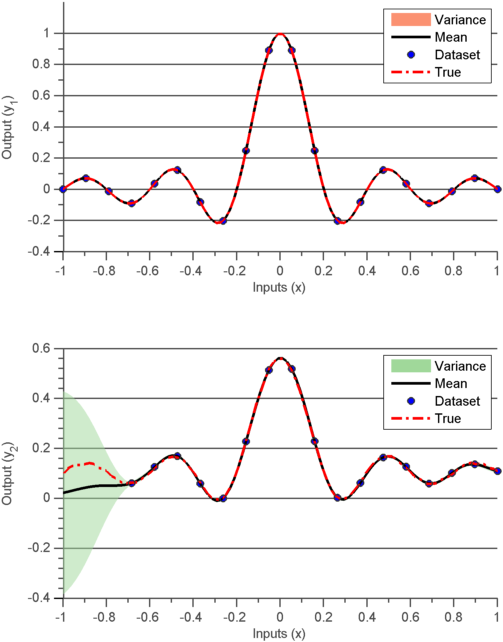
\includegraphics[width=0.29\textwidth]
        {images/part3/independentFitToyData}
        \label{subFigindependentFitToyData}
  }\quad
\subfigure[{GP posterior for a \textbf{simple multi-task} kernel conditioned on the data $\mathcal{D}_{4}$, we choose an SE kernel as the covariance across input points ($k_{inputs} = k_{SE}$). The points where data is unavailable has high value of variance but a better mean prediction when compared to figure \ref{subFigindependentFitToyData}}]
  {
        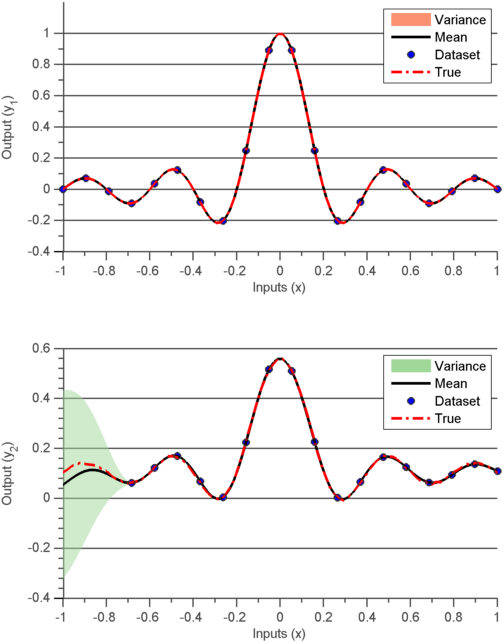
\includegraphics[width=0.29\textwidth]
        {images/part3/multiTaskFitToyData}
        \label{subFigmultiTaskFitToyData}
  }\quad
  \subfigure[{GP posterior for a \textbf{multi-fidelity} kernel conditioned on the data $\mathcal{D}_{4}$. We choose a SE kernel as the covariance across input points ($k_{inputs} = k_{SE}$) and covariance for $\delta$ process, the value of $r(x)$ is kept constant. We can observe that, the prediction at missing points is more accurate.}]
  {
        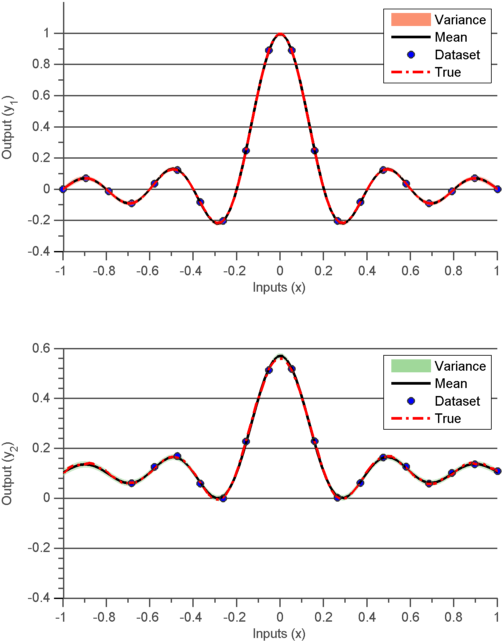
\includegraphics[width=0.29\textwidth]
        {images/part3/multiFidelityFitToyData}
        \label{subFigmultiFidelityFitToyData}
  }\quad

       \caption{Joint Posterior distribution for two outputs with missing data at $x^2 = [-1:-0.75]$. The solid black line defines the mean function, shaded region defines 95\% confidence interval (2$\sigma$) distance away from the mean.}
       \label{figJointPosteriorDistribution}
\end{figure}

\begin{mdframed}[hidealllines=true,backgroundcolor=lightgray!20]
We now compare the accuracy of the three methods for an increasing number of input points. To measure the accuracy of the prediction, we again use the 10-fold Cross Validation (CV).   

Figure \ref{subFigboxPlotsToyDataJoint} shows the accuracy of the three methods with an increasing number of data-points. The box-plots in red are cases when outputs are assumed independent, the box-plots in green are cases when covariance is assumed to be multi-task, and the box-plots in blue are cases when the output covariance is assumed to be multi-fidelity. As expected the error improves with the increasing number of data-points, the multi-fidelity covariance is best for all the three cases.
\end{mdframed}

\begin{figure}[!ht]
  \centering
    
        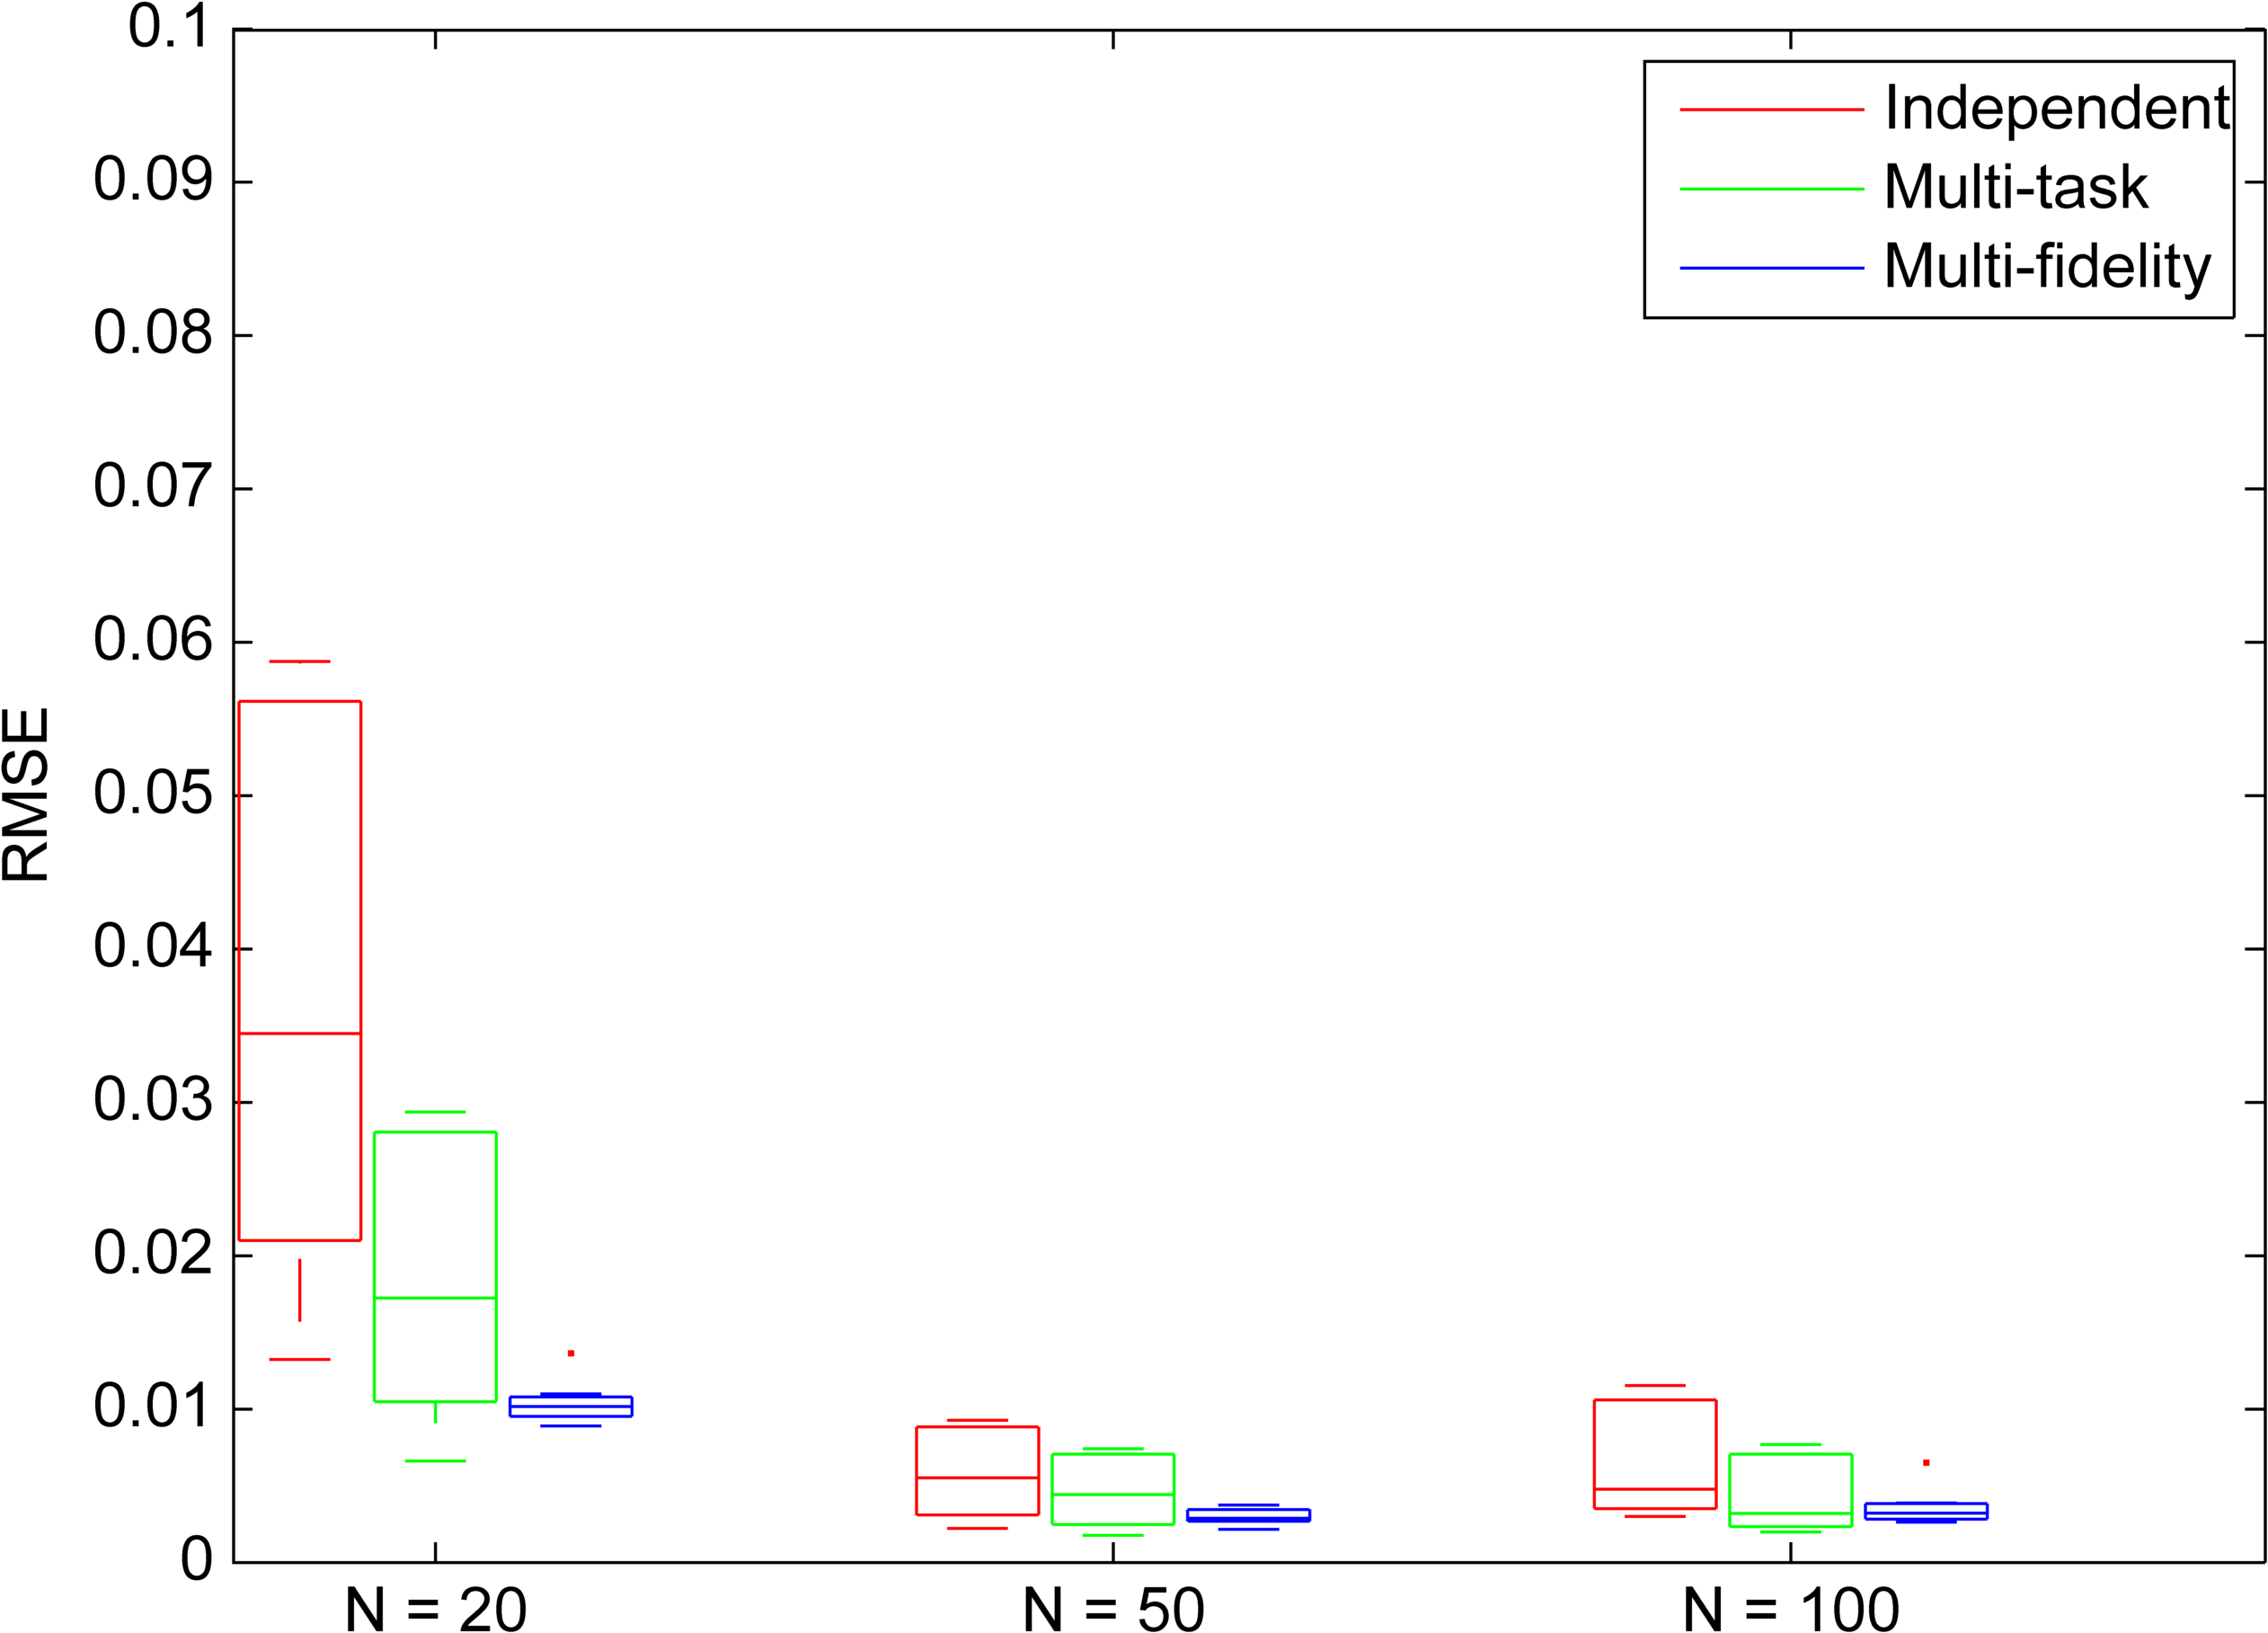
\includegraphics[width=0.45\textwidth]
        {images/part3/boxPlotsToyDataProgressionOverTime}
        \caption{10-fold RMSE box-plots for increasing number of input points. The box-plots in red are cases when outputs are assumed independent, the box-plots in green are cases when covariance is assumed to be multi-task, and the box-plots in blue are cases when the output covariance is assumed to be multi-fidelity. The error improves with increasing data-points,the multi-fidelity covariance is best fir for all the three cases.}
        \label{subFigboxPlotsToyDataJoint}
\end{figure}

\marginnote{\textsl{Linearly separable}}[1cm]
The independence assumption cannot learn the relationship between the outputs hence has the highest value of error. The multi-task covariance has better accuracy than the independent case, although it still cannot match the performance of the multi-fidelity model.  Multi-fidelity covariance model works so efficiently because the formula of the second output. The second output is a combination of a multiplication term to the first output $\textcolor{blue}{f^2/2}$, and a new term $\textcolor{red}{0.1cos(f^{1}(x))}$. This exactly matches the linearly separable assumptions in the multi-fidelity covariance function, on the other hand the multi-task model cannot effectively capture the new term $\textcolor{red}{0.1cos(f^{1}(x))}$.

\section{Extrapolation of Flight Loads}\label{subsecMTGPExtrapolation}
Once an aircraft design is ready and a flight-test aircraft is manufactured, it becomes the task of the aircraft manufacturer to certify the airplane. This section is dedicated to using GP algorithms to assist in the task of flight-loads certification. For certification of flight-loads, it is necessary to show that the loads (aerodynamic forces) experienced by the aircraft are coherent with the loads predicted during the design phase. To achieve this we perform flight tests with varying aircraft parameters and get a proper understanding of how the loads are varying with respect to various parameters.
\marginnote{\textsl{Certification}}[-1cm]

\marginnote{\textsl{Figure \ref{fig:flightLoadsDiagram}}}[1cm]
Figure \ref{fig:flightLoadsDiagram} is an example of the prediction of Shear Load (Tz) on a section of the wing, for varying values of Mach and Load factor (Nz). The points in blue are the points where tests have been performed, the black line denotes the convex hull of the flight test points. The 3d surface is the prediction of a GP model built by using measurements on the input points and an SE kernel. The boundaries denoted by the red lines are the limit load cases, flying near the limit conditions will result in irreversible damage to costly flight-test aircraft. The data is normalized according to Airbus standards.

\begin{figure}[ht!]
 \centering
 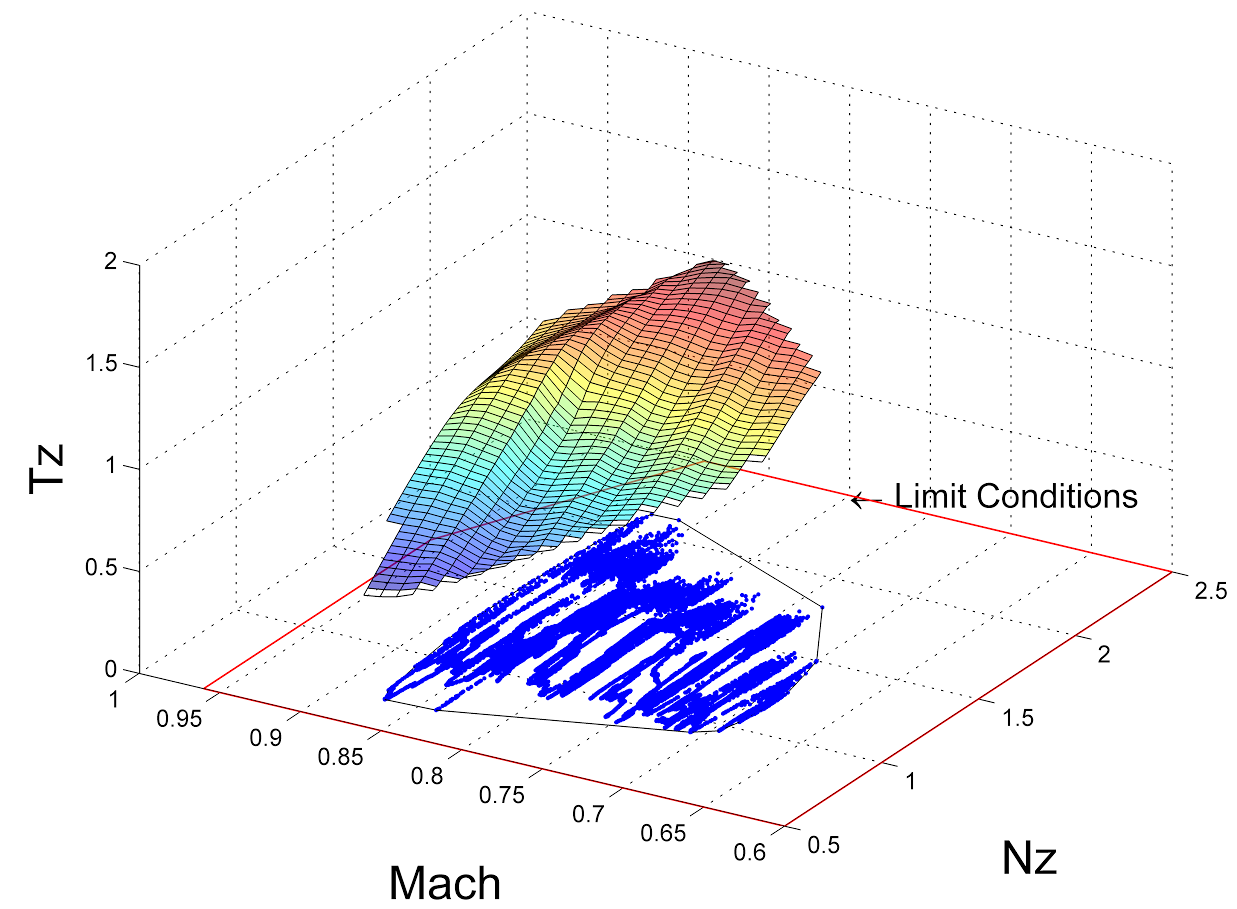
\includegraphics[width=0.75\textwidth]{images/part3/loadDomain}
 \caption{Flight-loads identification}
 \label{fig:flightLoadsDiagram}
\end{figure}

Verification and validation of the engineering model using experimental data of flight-test is a difficult exercise because:
\begin{enumerate}
\item Each flight-test campaign costs millions of euros, and hence flying the aircraft in all of the parameter combinations is very costly.
\item We cannot fly the aircraft at limit conditions because it will cause irreversible degradation to our single test-aircraft. But we still need to prove that the loads experienced at these limit conditions fall in the safety limit as prescribed by the certification authorities.
\end{enumerate}

Hence we need to both interpolate the experimental results in the convex hull of flight-test points, while also being able to extrapolate until the red line for certifying the safety limits. In this section, we propose a method to perform extrapolation using the engineering model developed during the detailed design phase. We would like to extend the MTGP formulation for extrapolation cases. 

\subsection{Current Approach}
\marginnote{\textsl{Theoretical loads model}}[1cm]
During the design phase of the aircraft, the flight loads department comes up with a theoretical model as shown in figure \ref{fig:currentFlightLoadsIdentificationApproach}. The aerodynamic department starts from a set of inputs comprising of aircraft states (for example angle of attack, Mach etc) and aircraft geometry (for example deformation of control surfaces), and runs CFD simulations on these set of inputs. Since we cannot run CFD simulations on each and every set of parameters in the flight domain, another aerodynamics team tries to build a parametric surrogate model which can map any set of aircraft states into rigid aerodynamic loads. This surrogate model is built by combining several types of aerodynamic computations, wind tunnel tests, and results in a lookup table model consisting of 100 aerodynamic parameters. In parallel the inertial loads department, uses the structural model to calculate the interial loads for same aircraft states. Finally, these two load models are combined to give the final load predictions. 

\begin{figure}[ht!]
 \centering
 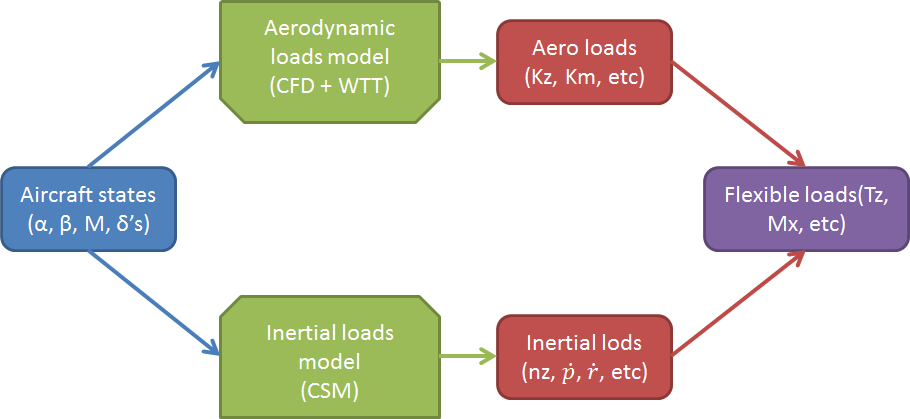
\includegraphics[width=\textwidth]{images/part3/flightLoadsModel}
 \caption{Current Flight-Loads theoretical model}
 \label{fig:currentFlightLoadsIdentificationApproach}
\end{figure}

\marginnote{\textsl{Complexity}}[1cm]
To update the simulation model, the measured data from flight-test is compared to the simulation predictions. The differences between the two models are minimized by minimizing the least square error. There are around 100 ($D_{outputs}$) load outputs (Tz, Mx, Kz etc), which are dependent on around 30 ($D_{input}$) flight parameters (Mach, the angle of attack etc). The parametric model has 100 variables and the flight tests are performed at millions of data-points. Updating this massively complex model is a highly complicated problem, requiring dozens of engineers and 6 months of certification time. Moreover, there are two main problems with this approach: 


\begin{enumerate}
\item Due to the parametric nature of the surrogate model, the updated model performs perfectly in certain areas of the flight domain while giving bad results in other parts. 
\item Due to the above issue many a times while updating the theoretical model, we add and remove certain parameters. Choosing which parameters to update and which parameters to add, requires a team of 5-10 engineers working for 6 months to finally deliver the updated model.
\end{enumerate}

\subsection{Proposed Approach}
\marginnote{\textsl{Non-parametric}}[1cm]
The main issue while using a parametric model is that, it uses parameters to express a function between input and outputs. This means to be able to express non-representable functions we iteratively add parameters in the model. We wish to replace this model updating phase with a MTGP model. We have access to both a relatively cheap simulation model produced during the design phase and costly flight-test experiments. Using the multi-fidelity formulation described in section \ref{secMTGP} we can encode the simulation model as a prior information. This helps in providing the correct bias and using the years of hard work encoded into the simulation model as a prior information for learning the flight-test model.

The figure, \ref{subFigmeasuredVssimulatedCl} shows a common example of the difference between a simulated model and an experimental model. It shows predictions of a simulated model of the coefficient of lift, with respect to the angle of attack (in green). The points in red denote the measurements from flight-test.  

% This again brings us into the multi-fidelity case, For the aircraft to be certified, the predictions of the simulation model should match the results of the flight-test phase. This is not always true since the simulation model is a representation of the true aircraft and contains several approximations and assumptions. 

\subsection{Proposed method}
There are currently three methods to perform extrapolation:
\begin{enumerate}
\item \textbf{Build a flight-test surrogate model}: We can build a GP model purely using data from flight-test. Unfortunately, the simple stationary covariance functions do not have any extrapolation capabilities (chapter \ref{chapBasicCovarianceKernels}). This means we would have to either use a Spectral Mixture to automatically detect patterns \cite{wilson2014thesis} or iteratively adjust the covariance function to detect patterns \cite{duvenaud-thesis-2014}. Unfortunately, flight-test data is very costly and thus we might not have access to a huge amount of data to learn detailed patterns. Moreover, by not using the information of a simulation model we are effectively putting years of hard-work into waste. 

\item \textbf{Update the simulation model}: This is the standard methodology used by design team during the certification process. The results of flight-test are compared to the results of prediction of a simulation model. A simulation model has several parameters, which are fine-tuned to decrease the difference between flight-test data and simulation results. This is a costly and time-consuming process, requiring a team of several dozen engineers working on a tight certification schedule. 

\item \textbf{Use multi-fidelity modelling}: The final option is using the multi-fidelity approach proposed in section \ref{secMultiFidelityMTGP}. If we assume the simulation model as a low-fidelity model, and flight-test data as results from a high-fidelity model, we can use launch the simulations at limit conditions and use the multi-fidelity formulation to perform predictions. This is equivalent to encoding the simulation model as the prior information. 
\end{enumerate}

\begin{mdframed}[hidealllines=true,backgroundcolor=blue!20]
Suppose we have a \(D_{inputs}\)-dimensional input space, and two outputs ($f^{s}$, $y^{e}$) which represent the simulation model and flight-test data respectively. The experiments are performed at the input points $x^{e}$ for $x^e \in \mathbb{R}^{N_{e} \times D_{inputs}}$, while the simulation model can be evaluated exactly at all points in the input domain.

\begin{equation}
    \Pr[f^{s}(x)] = GP(\bar{f^{s}(x)}, k^{s} = 0)
\end{equation}

Here, $\bar{f^{s}(x)}$ signifies evaluation of the simulation model at input point $x$, since the simulation model is deterministic the covariance term ($k^s$) is to zero. We can also signify the experimental observations as:

\begin{equation}
    y^{e}(x) = f^{e}(x) + \epsilon_{n_{e}} 
\end{equation}

Here, $f^{e}(x)$ is the latent physical process of the flight-test, while $\epsilon_{n_{e}}$ is experimental error. For the current case let's assume the experimental error is sampled from a white noise Gaussian , $\epsilon_{n_{e}} \sim \mathcal{N}(0, \sigma_{n_{e}}^2)$. We can therefore, write the joint prior between the experimental measurement ($y^{e}$) and simulation model ($f^{s}$) as:

\begin{equation}
\begin{aligned}
     \Pr \begin{bmatrix}
f^{s}\\ 
y^{e}
\end{bmatrix}  & = GP\left ( \begin{bmatrix}
\bar{f^{s}(x)}\\ 
r(x^{e})*\bar{f^{s}(x)}
\end{bmatrix}, \begin{bmatrix} k^{s}(x^{s}, x^{s}) & r(x^{s})k^{s}(x^{s}, x^{e})   \\
           r(x^{e})k^{s}(x^{e}, x^{s}) & r(x^{e})^2k^{s}(x^{e}, x^{e}) + k^{\delta}(x^{e}, x^{e}) + \sigma_{n_{e}}^2 \times I_{N_{e}}\end{bmatrix}   \right )
           \end{aligned}
\end{equation}

Since, the simulation model is deterministic, the covariance of the simulation model is zero ($k^s = 0$).

\begin{align}
\Pr \begin{bmatrix}
f^{s}\\ 
y^{e}
\end{bmatrix}    = GP \left ( \begin{bmatrix}
\bar{f^{s}(x)}\\ 
r(x^{e})*\bar{f^{s}(x)}
\end{bmatrix}, \begin{bmatrix} 0 & 0   \\
           0 & k^{\delta}(x^{e}, x^{e}) + \sigma_{n_{e}}^2 \times \mathbb{I}_{N_{e}}\end{bmatrix} \right ) 
\end{align}

Since the cross-covariance between simulation model and experimental data is zero, the two GPs are independent. We can thus write the GP prior for only the experimental data as equation \ref{eqIndependentGPExp}.

\begin{equation}\label{eqIndependentGPExp}
\Pr[y^{e}] = GP \left( r(x^{e})*\bar{f^{s}(x)}, \quad k^{\delta}(x^{e}, x^{e}) + \sigma_{n_{e}}^2 \times \mathbb{I}_{N_{e}} \right)
\end{equation}

The above form of the GP prior means that, the modified form of the simulation model can be treated as the mean of the GP prior, while the $k^{\delta}$ learns the difference between the two models. This result is exactly similar to recursive multi-fidelity model \cite{gratiet2012recursive} since we have broken the joint GP formulation into smaller parts. 

\marginnote{\textsl{Latency}}[1cm]
Often times when we are performing measurements we may have latency or translation among the measurements and predictions. This latency can be taken into account by introducing a delay hyper-parameter ($\Delta x$) \cite{osborne2008towards}. This means that our proposed prior can be written as:

\begin{equation}\label{eqProposedGPExp}
\Pr[y^{e}] = GP \left( r(x^{e} -\Delta x )*\bar{f^{s}(x - \Delta x)}, \quad k^{\delta}(x^{e}, x^{e}) + \sigma_{n_{e}}^2 \times \mathbb{I}_{N_{e}} \right)
\end{equation}

This is equivalent to assuming a Markov property as equation \ref{eqDelayedMarkovProperty}, $\forall x' \neq x - \Delta x$.

\begin{equation}\label{eqDelayedMarkovProperty}
         Cov(y^{i}(x), y^{i-1}(x') \mid y^{i-1}(x - \Delta x)) = 0
\end{equation}

If again we use a simple covariance function for $k^{\delta}$ then extrapolation of the covariance term will again tend to zero. This means that we still need to detect the pattern of the difference between experimental data ($y^e$), and simulation model ($r(x^{e} -\Delta x )*\bar{f^{s}(x - \Delta x)}$), but we have significantly reduced its need by applying the prior information of the simulation model. 
\end{mdframed}

\subsection{Experiments on toy data-set}\label{subsecExpToyDataset}
We now present a comparison of prediction accuracy between independent learning, multi-fidelity learning and proposed model in section \ref{secMultiFidelityMTGP}. We have used a elsA solver to simulate a NACA 0012 airfoil, the model uses SST turbulence model and the Coefficient of lift (Cl) values are measured at steady points. The points in green in figure \ref{subFigmeasuredVssimulatedCl} represent the results of the simulation for varying angle of attack, all the other variables (Mach, Reynolds number etc) are kept constant for this exercise. 

\begin{figure}[!ht]
  \centering
    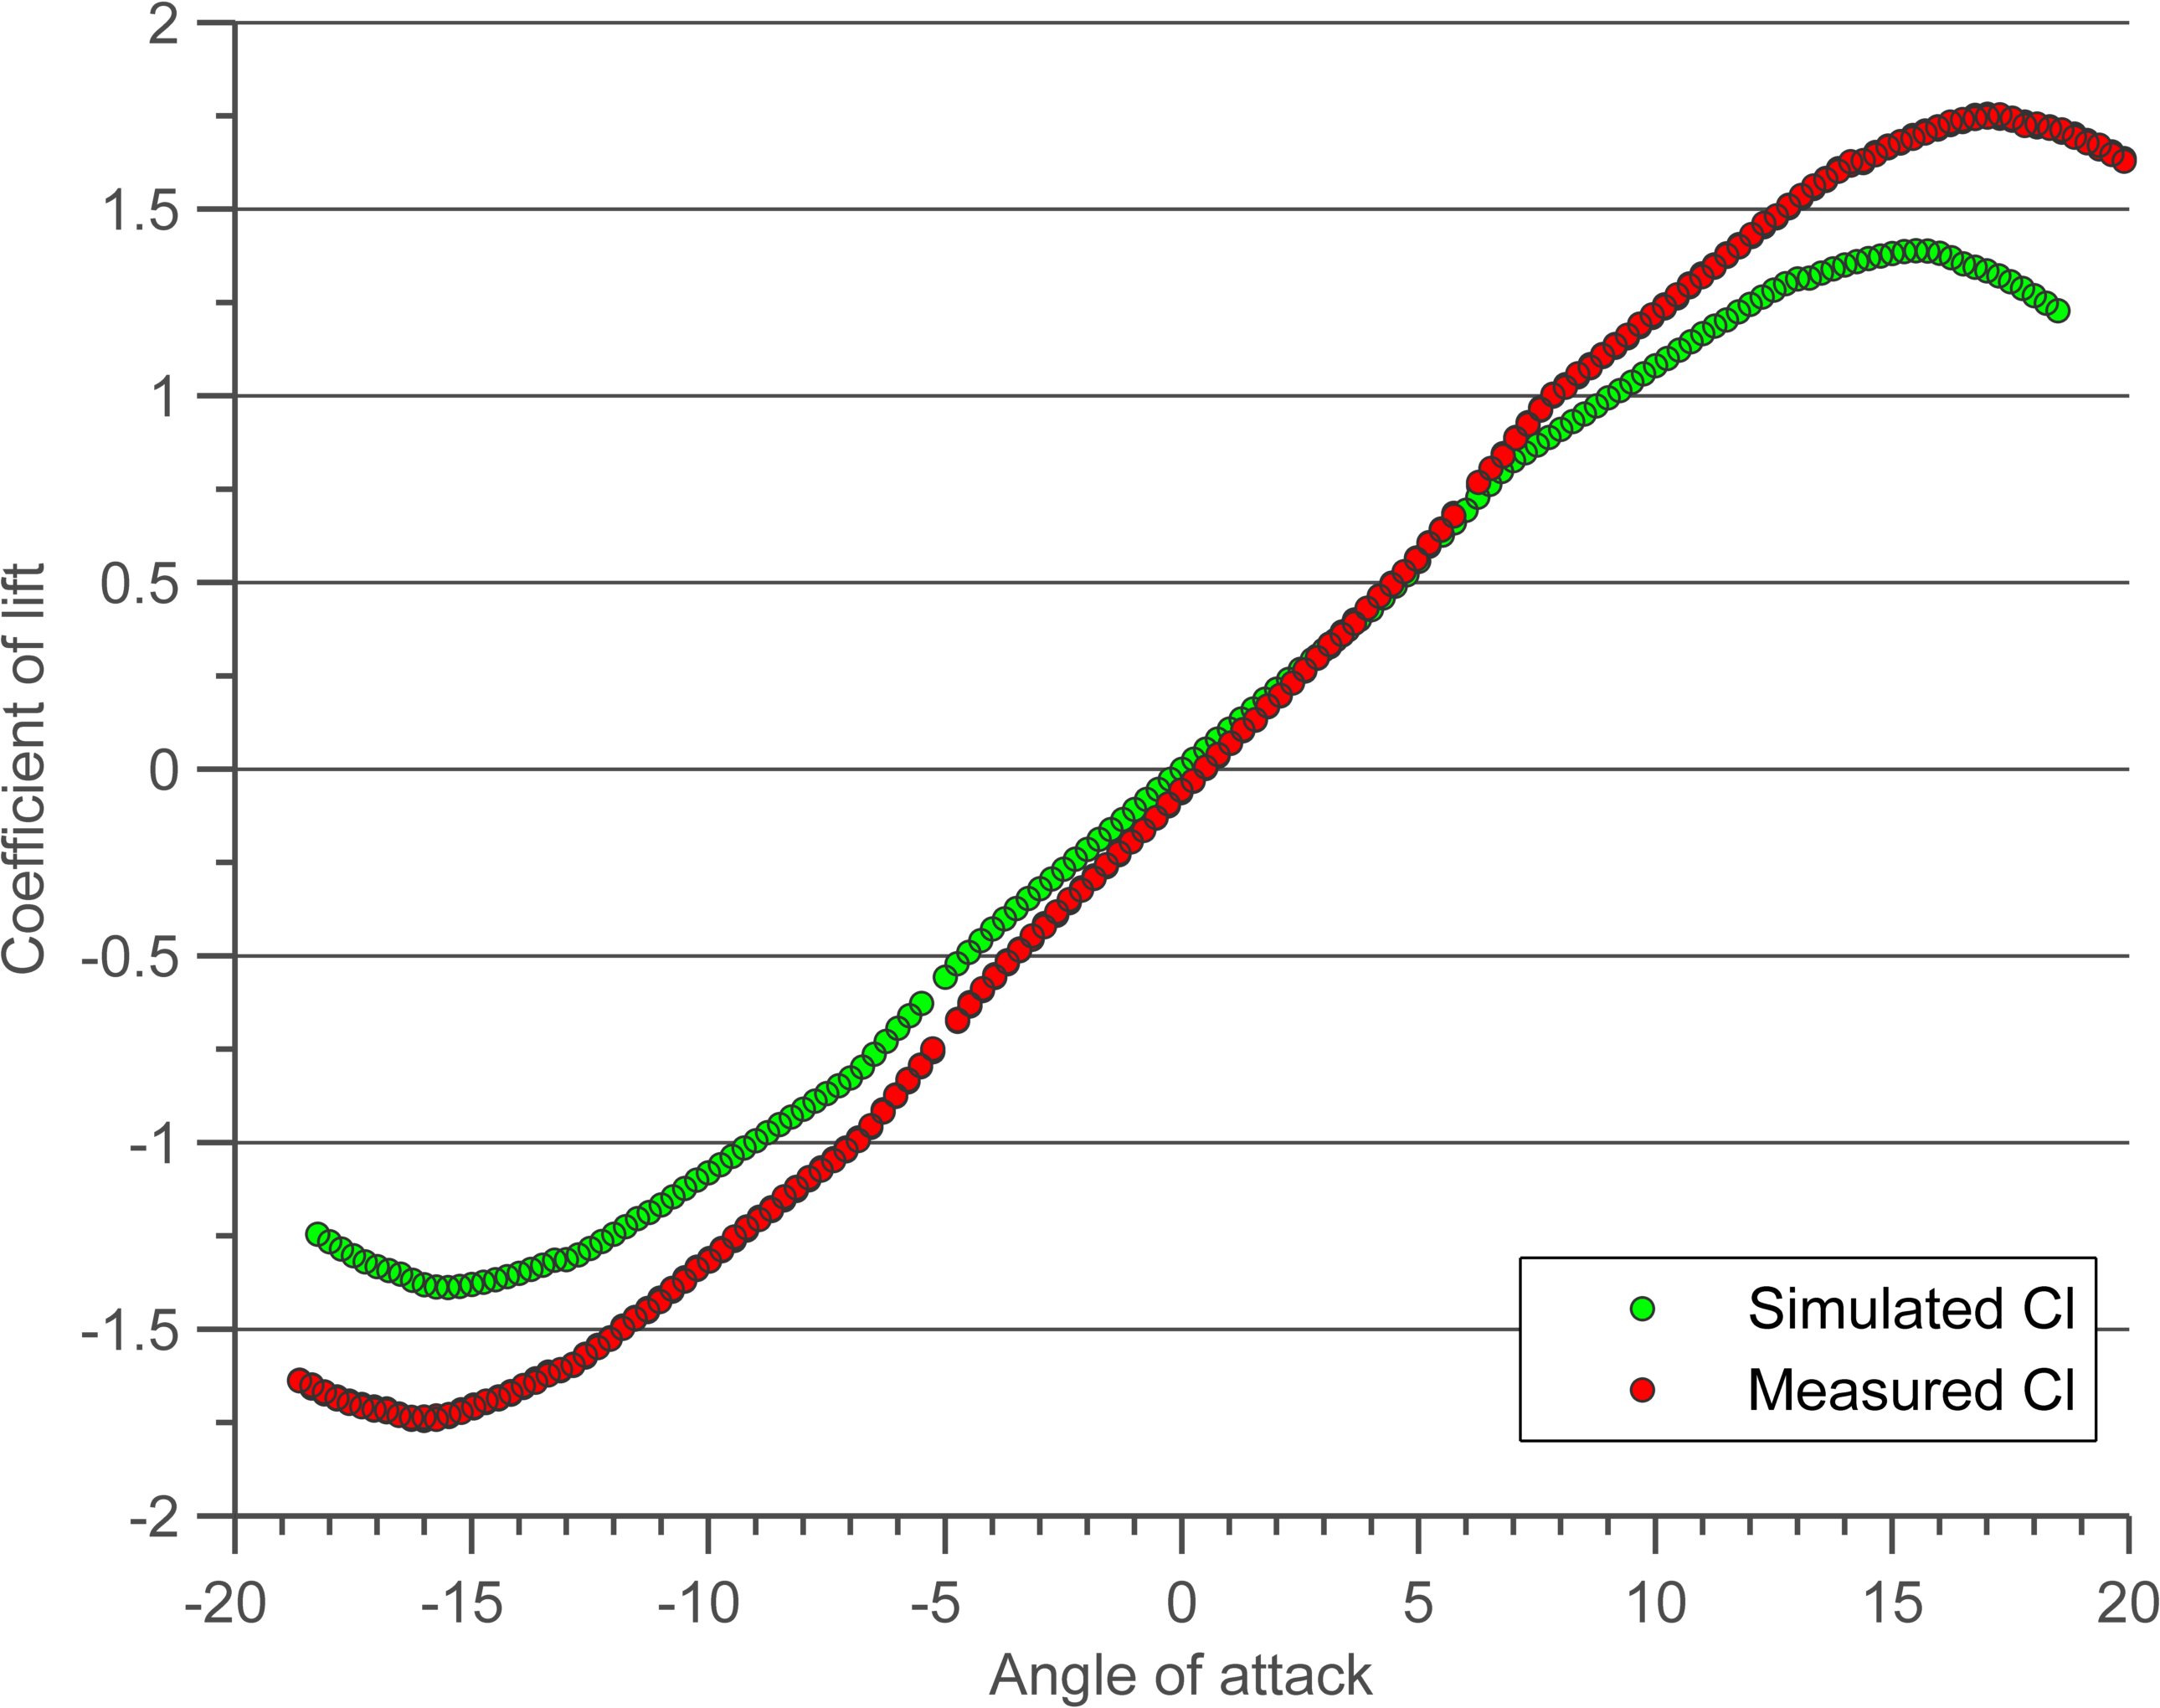
\includegraphics[width=0.45\textwidth]
        {images/part3/measuredVssimulatedCl}
        \label{subFigmeasuredVssimulatedCl}
       \caption{Example of difference between simulated Coefficient of lift ($f^s$) and experimental Coefficient of lift ($y^e$) (coming from equation \ref{eqSimpleModelWithTranslations}), with respect to angle of attack.}
\end{figure}

To represent the experimental data-set we make the following changes, equation \ref{eqSimpleModel} represents the case when there is no difference between experiment and simulation, equation \ref{eqSimpleModelWithError} represents the case when there is a measurement noise, equation \ref{eqSimpleModelWithSin} represents the case when the simulation has not captured a sinusoidal component in the measurements, and equation \ref{eqSimpleModelWithTranslations} represents the case when there is a translation in the measurement.  

\begin{align}
	y^{e}(x) & = f^{s}(x) \label{eqSimpleModel} \\
	y^{e}(x) & = f^{s}(x) + \epsilon_{n} \label{eqSimpleModelWithError} \\
	y^{e}(x) & = f^{s}(x) + sin(f^{s}) + \epsilon_{n} \label{eqSimpleModelWithSin} \\
	y^{e}(x) & = f^{s}(x + 0.2) + \epsilon_{n} \label{eqSimpleModelWithTranslations}
\end{align}

Here $\epsilon_{n}$ represents an independent noise, sampled from a white noise Gaussian $\epsilon_{n} \sim \mathcal{N}(0, 0.001)$. To measure the accuracy of predictions, we again launch a 10-Fold CV and calculate the RMSE. The 10-Fold CV has been performed for all the four types of changes between the measurement and experimental error. The hyper-parameters are fine-tuned for each of the three models (independent, multi-task and proposed model) by maximizing the marginal likelihood. 
\marginnote{\textsl{10-Fold CV}}[-1cm]

Figure \ref{figResultsOfExtrapolation} shows the box-plots of RMSE's for all the four cases. We see that the independent learning method always performs worst when compared to multi-task learning or proposed model with translations. When error starts appearing in the model then proposed model starts outperforming the multi-task method (there is no hyper-parameter for noise in the multi-task model). When there is a translation component present in the measurement then the proposed model clearly outperforms the two models.

\begin{figure}[!ht]
  \centering
        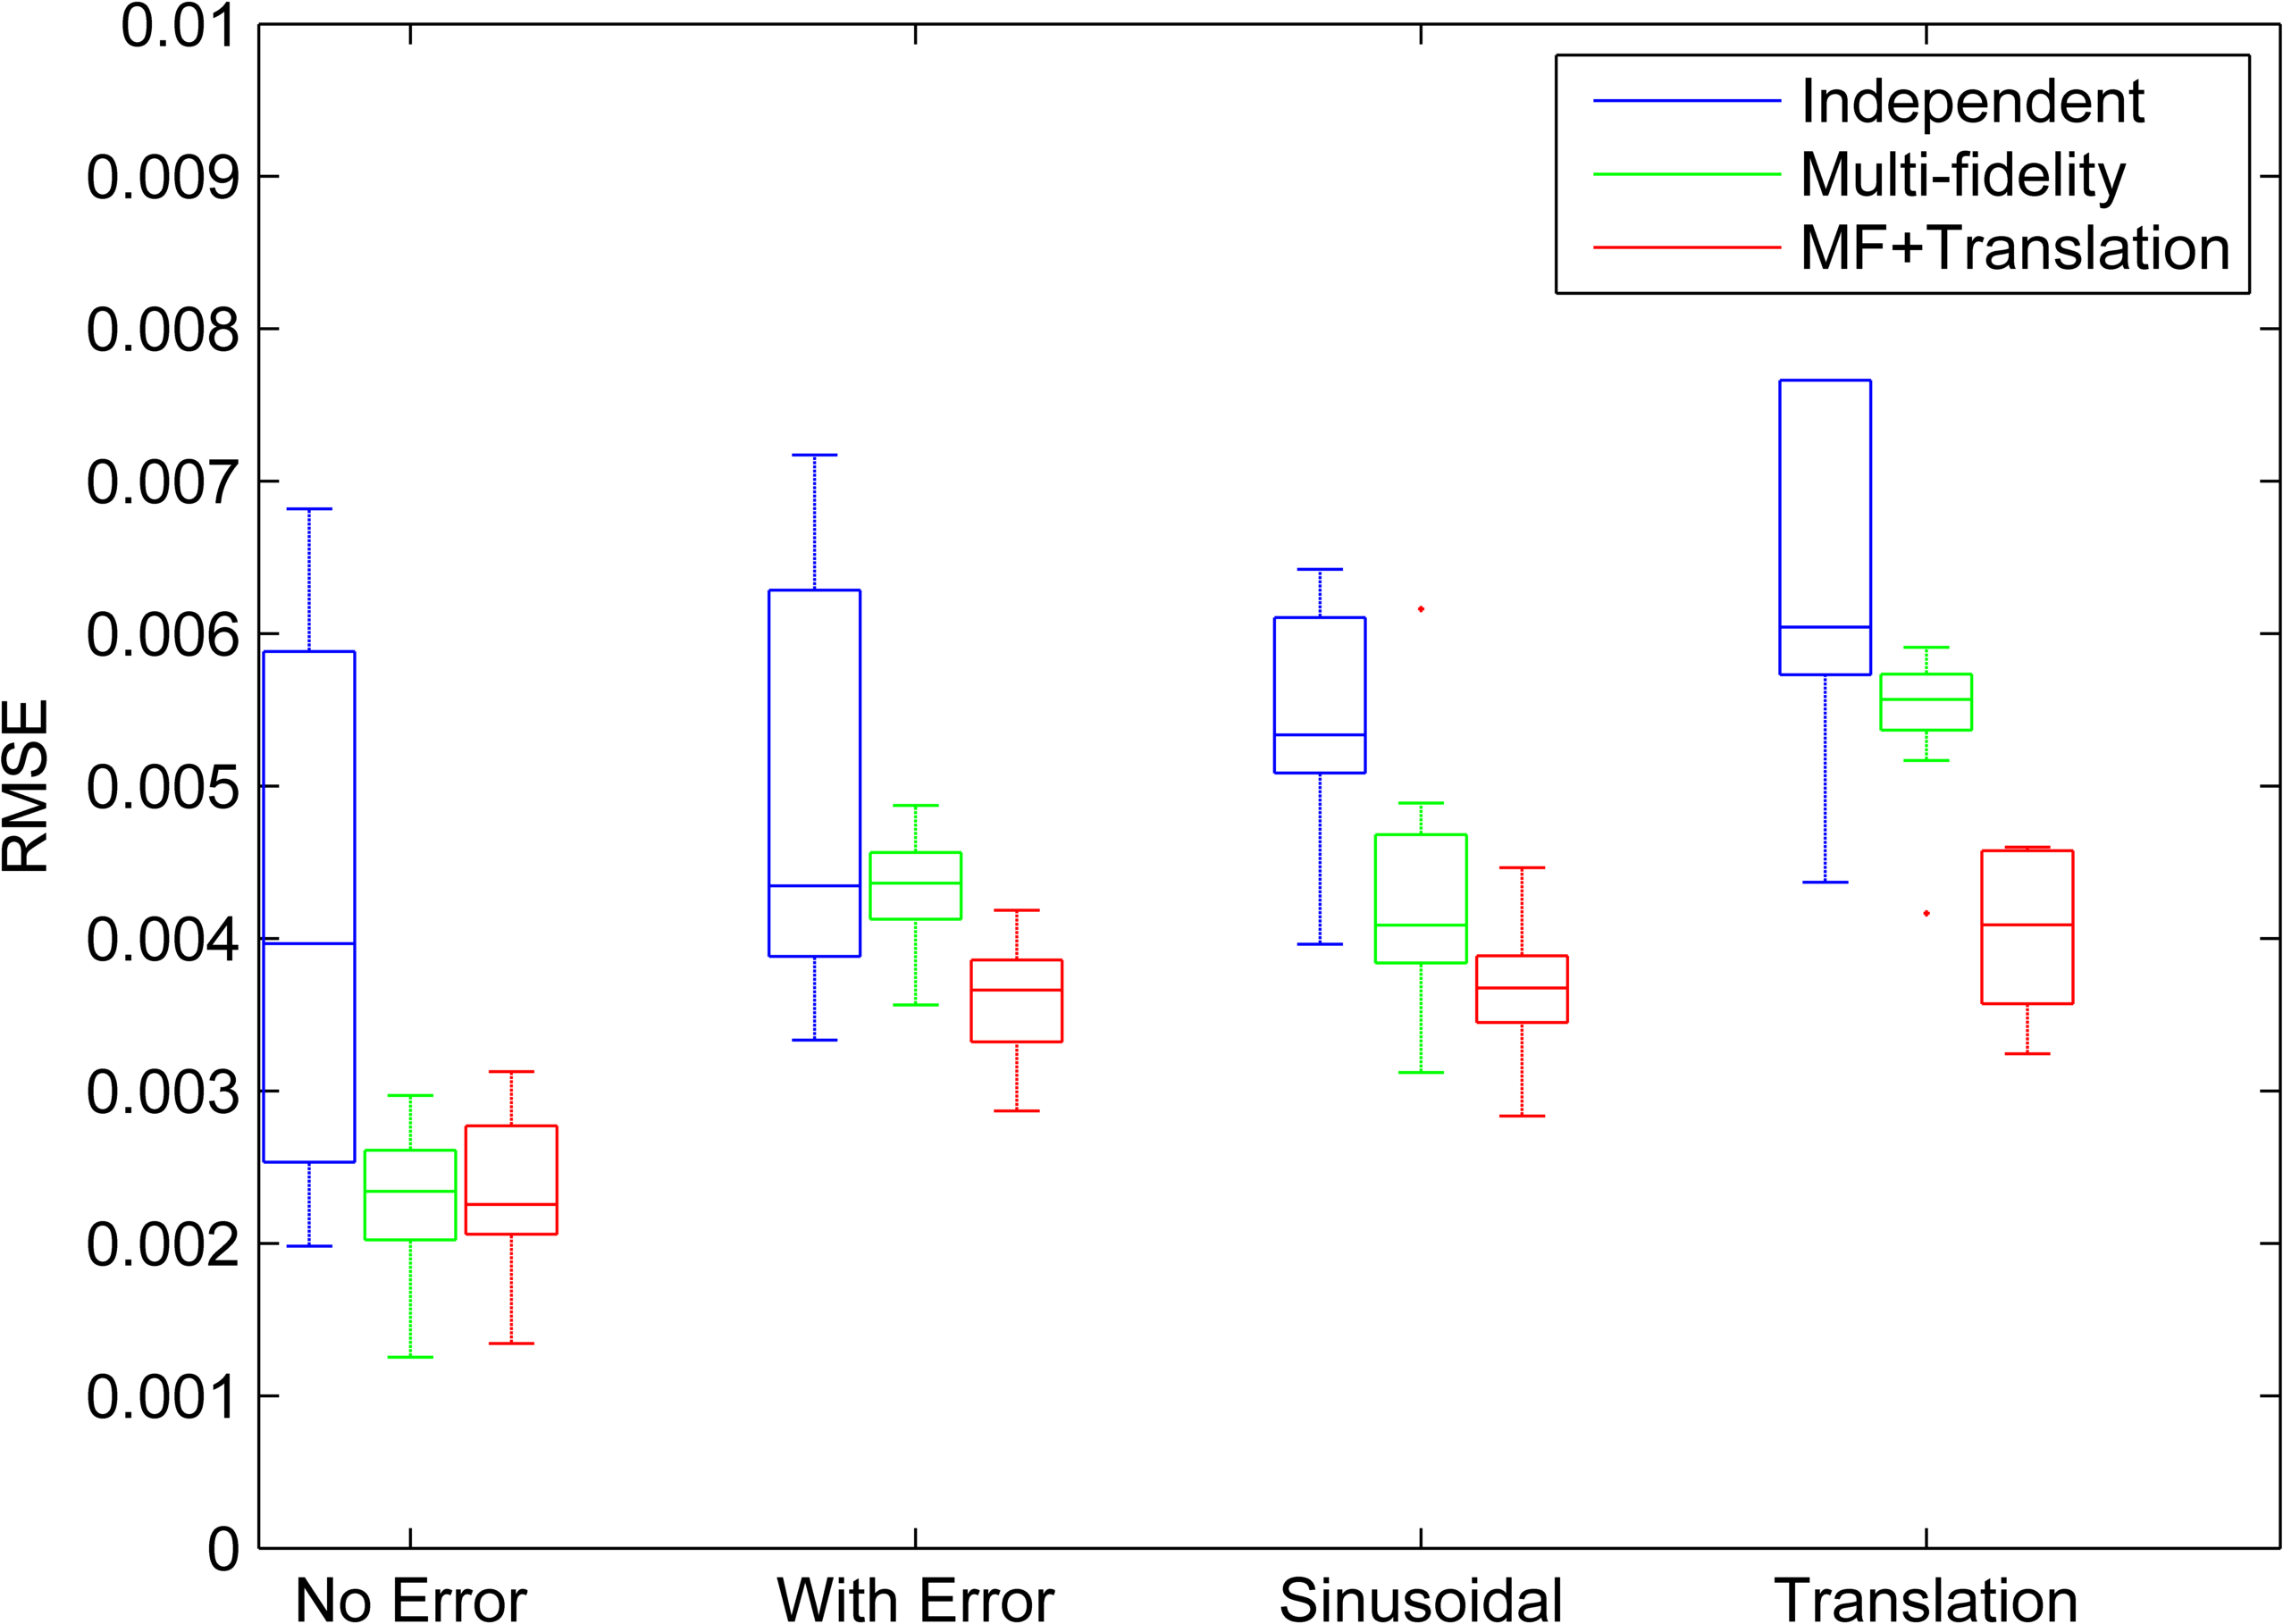
\includegraphics[width=0.45\textwidth]
        {images/part3/boxPlotsClAlphaAccuracyMeasure}
        \label{subFigboxPlotsClAlphaAccuracyMeasure}
       \caption{Boxplots of extrapolation for the four different cases; experimental set with no error (equations \ref{eqSimpleModel}), with a white noise error (equations \ref{eqSimpleModelWithSin}), with a sinusoidal error (equations \ref{eqSimpleModelWithSin}) and with translation (equations \ref{eqSimpleModelWithTranslations}). }
       \label{figResultsOfExtrapolation}
\end{figure}

The main aim of the current experiment is to present how the simulation model can be used for extrapolating experimental measurements. In our case, it is done by adding a translation hyper-parameter ($\Delta x$) to compensate for the lag in measurement and an error covariance to model the measurement error. We would also like to point out that the proposed model works better only because there is a translation term in the third case (equation \ref{eqSimpleModelWithTranslations}). 

\marginnote{\textsl{Non-separable}}[1cm]
Often times the different models cannot be linearly separable by the Markov property. This leaves us with three choices, we can try and identify the pattern in experimental data by using pattern detecting covariance functions \cite{wilson2014thesis}. Second, we can use a non-separable MTGP joint-covariance to learn the relation between the simulation model and the experimental model \cite{alvarez2011kernels}, or third, we can learn the pattern of the $k^\delta$ automatically \cite{duvenaud2013structure}. We wish to study the prediction properties of all the three proposed approaches and try to understand which is the better choice for tasks of model updating and extrapolation in the future.


\section{Summary and discussion}
In the current chapter, we have seen how to perform GP regression in the presence of multiple outputs. One simple method of learning a regression model for multiple outputs is by assuming the output number as an extra dimension (this extra dimension is a categorical variable). This observation is beneficial due to two reasons, first, we have effectively increased the number of data-points (figure \ref{figoutputsAsAnExtraDimension}). Second, all the tricks of making covariance functions for multiple dimensions can be applied to the case of multiple outputs as well (section \ref{subsecAnExtraDimension}). 

If no information is available about the relation between outputs then we can learn the relationship between outputs by either using a simple MT covariance (section \ref{simpleMultiTask}), a `Linear Model of Coregionalization' (section \ref{subsecLMC}), or a convoluted GP \cite{alvarez2011kernels}. If we know \textit{a-priori} that the outputs are coming from models of multiple fidelity then we can use the joint covariance function proposed by  \cite{kennedy2000predicting} (section \ref{secMultiFidelityMTGP}). 

In section \ref{subsecMTGPExtrapolation} we have shown how multi-fidelity GP models can be used to perform interpolation or extrapolation of experimental data. We include an error term and a translation term into a normal multi-fidelity model to account for differences in the simulation model and experimental data. In the future, we would wish to quantify the performance of different methods of extrapolation and decide which method to choose in a particular scenario.
